\RequirePackage[dvipsnames]{xcolor}
\documentclass[10pt]{NSP1}
\usepackage{url,floatflt}
\usepackage{helvet,times}
\usepackage{psfig,graphics}
\usepackage{mathptmx,amsmath,amssymb,bm}
\usepackage{graphicx}
\usepackage{booktabs}
\usepackage{multirow}
\usepackage{float}
\usepackage{tabularx}
\usepackage{array}
\usepackage{enumitem}
\usepackage{stfloats}
\usepackage[bf,hypcap]{caption}

% Float placement & spacing optimizations
\renewcommand{\topfraction}{0.95}
\renewcommand{\bottomfraction}{0.95}
\setcounter{topnumber}{4}
\setcounter{bottomnumber}{3}
\setcounter{totalnumber}{6}
\setcounter{dbltopnumber}{4}
\renewcommand{\dbltopfraction}{0.95}
\renewcommand{\textfraction}{0.05}
\renewcommand{\floatpagefraction}{0.8}
\renewcommand{\dblfloatpagefraction}{0.8}

\setlength{\textfloatsep}{5pt plus 1pt minus 1pt}
\setlength{\floatsep}{4pt plus 1pt minus 1pt}
\setlength{\intextsep}{4pt plus 1pt minus 1pt}
\setlength{\dbltextfloatsep}{5pt plus 1pt minus 1pt}
\setlength{\dblfloatsep}{4pt plus 1pt minus 1pt}

\captionsetup{
	aboveskip=3pt,
	belowskip=2pt
}

\setlist{nosep,leftmargin=*}

\tolerance=1
\emergencystretch=\maxdimen
\hyphenpenalty=10000
\hbadness=10000

\topmargin=0.00cm

\def\sm{\smallskip}
\def\no{\noindent}

% Abbreviations
\def\feo{\ensuremath{\mathrm{Fe}_3\mathrm{O}_4}}

\def\firstpage{1}
\setcounter{page}{\firstpage}
\def\thevol{1}
\def\thenumber{1}
\def\theyear{2026}

\begin{document}
	
	\titlefigurecaption{{\large \bf \rm \vspace{0.15cm}International Journal of Thin Films Science and Technology }{}}
	
	\title{Nanoparticle--Blood Flow and Immune System Interactions in Advancing Cardiovascular Health: A COMSOL Multiphysics Analysis}
	
	\author{Sahin Ahmed$^1$, Anil Nangkar$^2$ and Kottakkaran Sooppy Nisar$^{3,4,5,*}$}
	\institute{$^{1,2}$Department of Mathematics, Rajiv Gandhi University, 791112, Arunachal Pradesh, INDIA\\
		$^3$Department of Mathematics, College of Science and Humanities, Prince Sattam bin Abdulaziz University, KSA\\
		$^4$Mathematics Research Center, Near East University, 99138 Nicosia, Turkey\\
		$^5$Hourani Center for Applied Scientific Research, Al-Ahliyya Amman University, Amman, Jordan}
	
	\titlerunning{Nanoparticle--blood flow and immune system interactions}
	\authorrunning{S. Ahmed, A. Nangkar, K.S. Nisar}
	
	%corresponding author email
	\mail{ksnisar1@gmail.com}
	
	\abstracttext{This paper provides an elaborate mathematical model for the association between the flow of blood in arteries, WBCs, cytokines, and nanoparticles in regulating vascular inflammation. What makes this research stand out is the integration of hemodynamics, transport in immunology, and physical attributes of nanoparticles into a computational model used for treating cardiovascular diseases. The study adopts COMSOL Multiphysics platform in investigating the effect of nanoparticles on the functions of the immune system through reaction-convection-diffusion equations. This model clarifies the role of particles in interactions with cytokines and WBCs, thus improving the efficacy of the delivery process of nanoparticles to the region of inflammation. Results showed that magnetically activated \feo\ particles significantly increased WBCs' reaction at inflamed sites. On the other hand, SWCNT particles were characterized by higher thermal conductivity but failed to cause any change in chemotactic reactions. This aspect is particularly crucial when designing new precision medicine approaches to manage inflammatory-related cardiovascular disease, such as atherosclerosis. The proposed computational method has successfully contributed to solving the knowledge gap that exists while offering a strong framework for future work in this regard.}
	
	\keywords{Blood flow, White blood cell, COMSOL Multiphysics, Nanoparticles, MHD.}
	
	\maketitle
	
	\section{Introduction}
	
	Cardiovascular diseases present significant mortality and morbidity worldwide. Characterizing arterial blood flow patterns is fundamental to diagnosing and treating these conditions. In this study, we investigate the contributions of WBCs and cytokines to the inflammatory pathways activated in multifaceted vascular pathologies. Inflammation is central to the pathophysiology of many diseases, including atherosclerosis. In atherosclerosis, some cytokines control the immune response, and WBCs are recruited to the inflamed endothelium. This model also examines the use of engineered nanoparticles for the modulation of these biological responses to augment the delivery and enhance the therapeutic effects of treatments. This work combines advanced computational modeling with the complexities and interrelated functionality of arterial blood flow, WBCs, cytokines, and nanoparticles. With the use of COMSOL Multiphysics, these simulations strive to elucidate new perspectives toward therapeutic vascular improvement.
	
	Understanding arterial blood flow velocity and health has significant implications on the aging process and countless other conditions such as atherosclerosis. Hemodynamic forces and shear stress act on the endothelium, which is susceptible to plaque buildup. Low shear stress correlates with a tendency for plaque buildup \cite{Ku1997}. More sophisticated models such as those proposed by Zhao et al.\ \cite{Zhao2000} and Steinman \cite{Steinman2004} have the ability to predict the progression of a given pathology. The work of Singh et al.\ \cite{Singh2010} and Rezazadeh and Ostadi \cite{Rezazadeh2022} shows the potential of imaging and modeling to examine the complex phenomena that occur in constricted arteries. Katanov et al.\ \cite{Katanov2015} studies microvascular blood flow resistance, and red blood cell migration and dispersion, which are crucial phenomena of microcirculation. Milnor \cite{Milnor1989} and Iliceto et al.\ \cite{Iliceto1991} provided fundamental insights into cardiovascular hemodynamics and blood-flow velocity measurements under physiological conditions.
	
	Nanoparticles are considered one of the important facets of nanotechnology with great applications in the biomedical domain. Nanoparticle applications have been found in various aspects, including the development of nanoparticle-based drug delivery systems and nanoparticle-based diagnostic approaches. For instance, according to Shen et al.\ \cite{Shen2018}, there have been investigations regarding biocompatibility and magnetism of \feo\ nanoparticles for targeted therapies. As per Fullstone et al.\ \cite{Fullstone2015}, SWCNTs are discussed along with the special electric and thermal characteristics of such particles for enabling delivery mechanisms and temperature control. The ability of nanoparticles to follow diverse routes in the blood flow is well established by previous research conducted by Gentile et al.\ \cite{Gentile2008} and Ghasemi et al.\ \cite{Ghasemi2015}. Another study by Boujelbene et al.\ \cite{Boujelbene2023} analyzes the thermal and mechanical impacts of nanoparticles under a magnetic field. Siogkas et al.\ \cite{Siogkas2011} developed patient-specific multiscale arterial models, demonstrating the usefulness of computational approaches in cardiovascular disease analysis.
	
	A synergistic relationship between white blood cells (WBCs) and cytokines in circulation is critical for a strong immune response, especially during inflammation. This is evidenced by research done by Gerhardt and Ley \cite{Gerhardt2015} and Cavaillon \cite{Cavaillon1994}, where they demonstrate how cytokine signalling is involved in coordinating the actions of WBCs and consequently guides their mobility and effectiveness. In turn, it is possible for nanoparticles to change these dynamics in ways that can strengthen immune response, which has been demonstrated by Zlotnik and Yoshie \cite{Zlotnik2000} and Dubey et al.\ \cite{Dubey2021}. Such alterations present an avenue for improving targeting and effectiveness of immunotherapy, especially those involving the vasculature. Khan and Khan \cite{KhanKhan2009} emphasized the crucial role of white blood cells and cytokine-mediated signaling in regulating immune responses during inflammation. Hewlin et al.\ \cite{Hewlin2023} study the impact of unstable flows on the targeting effectiveness of magnetic nanoparticles in arterial stents. Anderson et al.\ \cite{Anderson2013} and Lee et al.\ \cite{Lee2010} reported that nanoparticle diffusion, size, and targeting characteristics significantly influence transport efficiency and biodistribution in biological systems. Sha et al.\ \cite{Sha2017}, Wei et al.\ \cite{Wei2018}, and Muhammad et al.\ \cite{Muhammad2018} highlighted the superior magnetic responsiveness of \feo\ nanoparticles and the excellent thermal conductivity of SWCNTs, making them attractive for biomedical transport applications.
	
	The role of computational modelling in cardiovascular research is vital in that it facilitates the construction and forecasting of complex interactions in the cardiovascular system. Budu-Grajdeanu et al.\ \cite{Budu2008} and Cilla et al.\ \cite{Cilla2014} make use of computational methods to model disease processes and possible treatment options. Advances in computation methods highlighted by Menon et al.\ \cite{Menon2024} and Ali et al.\ \cite{Ali2021} enable the creation of complex multiscale models that accurately represent physiological systems. Fractional modelling of MHD blood flow along with the introduction of magnetic particles for improved visualization and targeting within vascular models has been addressed by Majeed et al.\ \cite{Majeed2022}. Blood flow mechanics have also been studied by other scholars, such as Vaidya et al.\ \cite{Vaidya2021} and Ougrinovskaia et al.\ \cite{Ougrinovskaia2010}. Ahmed and Mishra \cite{AhmedMishra2026} developed a semi-experimental model via COMSOL Multiphysics to investigate the behaviour of stenosis height in a stenotic artery to simulate blood flow containing microorganism and silver nanoparticles under the influence of Reynolds number, Hartmann number, and bioconvection Lewis number. The classical models of Maxwell \cite{Maxwell1873} and Brinkman \cite{Brinkman1952} remain widely used for estimating the effective thermal conductivity and viscosity of nanoparticle suspensions.
	
	In this investigation, we introduce a numerical model using governing equations in conjunction with blood mass transport for studying the interplay between white blood cells, cytokines, and synthetic nanoparticles. Based on an extensive review of the relevant literature, this model is able to fill the critical gap in scientific knowledge by investigating the regulation of immune system responses within the cardiovascular system. The parameters, such as reaction rate constants and diffusivity coefficients, are precisely computed based on experimental data available in the literature to make sure that the simulation outputs mimic real biological processes. Through focusing on this relationship, the main aim of this model is to provide us with new insights into the effectiveness of nanoparticle therapy.
	
	\section{Model hypothesis}
	
	The present research paper aims at developing the concept of chemotactic motion of white blood cells (WBCs) under the influence of nanoparticle-cytokine interactions along with a magnetic field acting on the moving blood in the artery. The computational domain consists of a three-dimensional simulation of a blood vessel enclosed by the inflow and outflow boundaries, whereas there exists an infected area on the surface of the blood vessel that constantly secretes cytokines into the surrounding environment. This local secretion of cytokines acts as a stimulus for the attraction of WBCs towards the affected zone, which imitates inflammatory behaviour of the immune system.
	\newpage
	\begin{figure}[!htbp]
		\centering
		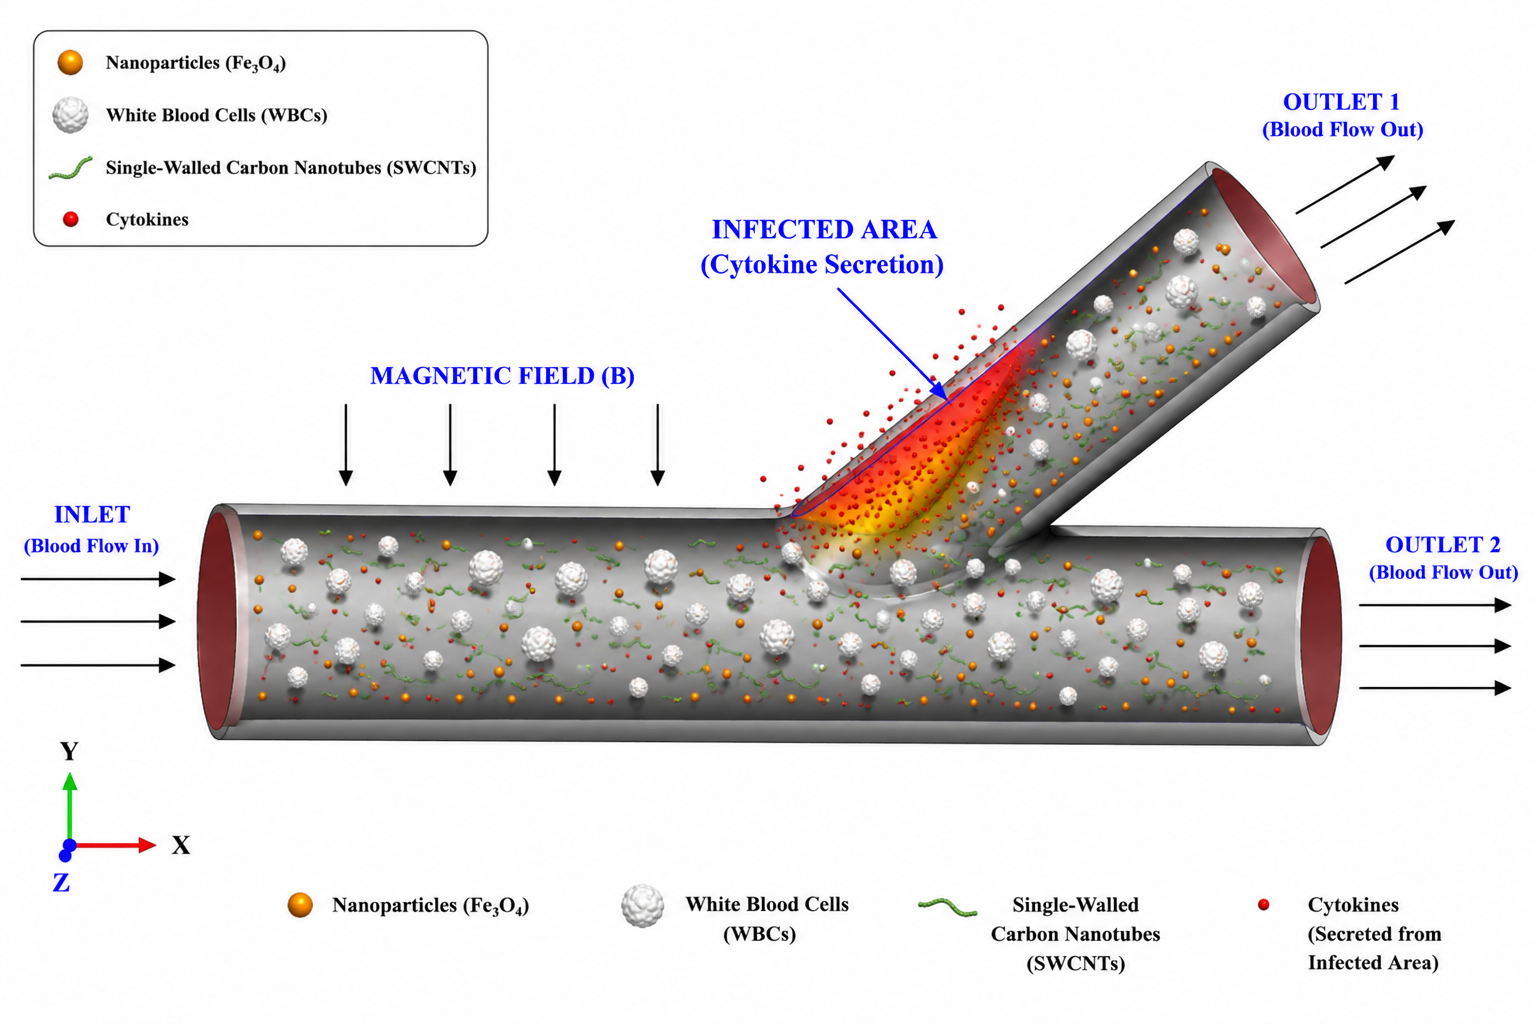
\includegraphics[width=0.88\columnwidth]{fig1_schematic.png}
		\caption{2D Schematic diagram of the model.}
		\label{fig:schematic}
	\end{figure}
	
	The geometry is structured to replicate arterial dimensions, suitable for laminar, steady blood flow. Blood is treated as an incompressible, Newtonian fluid with constant density ($\rho_{f}$) and dynamic viscosity ($\mu_{f}$). Under these assumptions, the model adheres to a steady, laminar flow profile, aligning with physiological conditions in medium to small blood vessels. There exist two types of nanoparticles, which include \feo\ (magnetite) and SWCNT (Single-Walled Carbon Nanotube). These are injected into the bloodstream in order to investigate their various influences in terms of the migration of white blood cells (WBCs) due to the presence of magnetic forces. Under the current context, WBC locomotion occurs through the mechanism of chemotaxis in response to the cytokine concentration gradient within the infected region. The underlying mathematics behind this model takes into consideration these interactions where the WBC density acts as the chemotactic variable, while nanoparticle density affects WBCs depending on magnetic variations. Building upon that, the present model aims to address the following research questions:
	\begin{enumerate}[label=\arabic*.]
		\item How does $\chi$ impact the temporal and spatial accumulation of WBCs in response to cytokine gradients, particularly in inflamed regions?
		\item What is the influence of \feo\ nanoparticles and SWCNTs on WBC migration and temperature modulation under changing magnetic field conditions, and how do their properties shape therapeutic outcomes?
		\item Can magnetic field modulation augment the sensitivity of WBCs to cytokine gradients, and what character do \feo\ nanoparticles play in strengthening this impact compared to SWCNTs?
		\item What are the thermal and chemotactic performance differences between \feo\ and SWCNT nanoparticles, and how can their distinct behaviours under magnetic influence be optimized for targeted therapeutic interventions?
		\item How does the interaction between WBCs, cytokines, and nanoparticles change with time according to different levels of chemotactic sensitivities and magnetic fields? What are the consequences of such interaction on the accuracy of targeted immune treatments?
	\end{enumerate}
	
	\section{Governing equations}
	
	The system of equations which describe the blood flow, temperature profile, movement of nanoparticles, WBCs, and cytokine concentration can be found below. The set of equations for each of the cases is provided together with respective boundary conditions used in the COMSOL simulation.
	
	\subsection{Blood flow along the vessel}
	\label{sec:bloodflow}
	
	Blood flow is considered as an incompressible, Newtonian fluid, described by the continuity and Navier-Stokes equations. The continuity equation ensures the conservation of mass:
	\begin{equation}\label{eq:continuity}
		\nabla\cdot u = 0,
	\end{equation}
	and the Navier-Stokes equation governs momentum conservation \cite{Ku1997,Steinman2004}:
	\begin{equation}\label{eq:navierstokes}
		\frac{\partial u}{\partial t} + (u\cdot\nabla)u = - \frac{1}{\rho_{nf}}\nabla p + \frac{\mu_{nf}}{\rho_{nf}}\nabla^{2}u + \frac{1}{\rho_{nf}}(J \times B),
	\end{equation}
	where:
	\begin{itemize}
		\item $u$ is the velocity vector field,
		\item $\rho_{nf}$ is the density of nanofluid,
		\item $\mu_{nf}$ is the dynamic viscosity,
		\item $p$ is the pressure,
		\item $J,B$ represent the electric current density and the applied magnetic field.
	\end{itemize}
	
	At the inlet, a velocity profile is applied to simulate physiological blood flow conditions, ensuring a realistic representation of blood entering the vessel. The outlet boundary condition adopts an outflow profile ($n \cdot \nabla p = 0$) to maintain continuity of flow without artificial pressure buildup. Vessel walls are modelled with no-slip conditions ($u = 0$), accurately representing the frictional interaction between blood and the endothelial surface.
	
	\subsection{Nanoparticle transport}
	\label{sec:nanoparticle}
	
	Nanoparticles (\feo\ and SWCNT) are transported within the bloodstream according to the convection-diffusion equation \cite{Gentile2008,Fullstone2015}:
	\begin{equation}\label{eq:np}
		\frac{\partial C_{np}}{\partial t} + \nabla\cdot\left( uC_{np} \right) = D_{np}\nabla^{2}C_{np},
	\end{equation}
	where:
	\begin{itemize}
		\item $C_{np}$ is the nanoparticle concentration,
		\item $D_{np}$ denotes the diffusion coefficient of nanoparticles.
	\end{itemize}
	
	At the inlet, the concentration of nanoparticles is defined by the volume fraction, $\phi$, representing the initial distribution of nanoparticles in the bloodstream. This volume fraction can be adjusted based on experimental or simulation needs. The outlet follows a convective flux condition $(n\cdot D_{np}\nabla C_{np} = 0)$, allowing nanoparticles to exit the domain naturally with the flow. The vessel walls are modelled with a no-flux condition to prevent nanoparticle loss through the vessel boundaries.
	
	\subsection{WBC transport and Chemotaxis}
	\label{sec:wbc}
	
	The migration and distribution of WBCs within the flow are influenced by both convection-diffusion equation and chemotaxis \cite{Zlotnik2000,Gerhardt2015}:
	\begin{equation}\label{eq:wbc}
		\begin{split}
			\frac{\partial C_{WBC}}{\partial t} + \nabla \cdot (uC_{WBC}) ={} & D_{WBC}\nabla^{2}C_{WBC}\\
			&- \chi\nabla \cdot (C_{WBC}\nabla C_{cytokine}),
		\end{split}
	\end{equation}
	where:
	\begin{itemize}
		\item $C_{WBC}$ is the concentration of WBCs,
		\item $D_{WBC}$ is the WBC diffusion coefficient,
		\item $\chi$ represents the chemotactic sensitivity coefficient indicating the response strength of WBCs to cytokine gradients,
		\item $C_{cytokine}$ is the cytokine concentration.
	\end{itemize}
	
	The chemotactic term, $-\chi\nabla \cdot (C_{WBC}\nabla C_{cytokine})$, represents the directed movement of WBCs toward higher cytokine concentrations. This term reflects the natural biological response where WBCs are attracted to sites of infection or inflammation, following the cytokine concentration gradient. At the inlet, a baseline concentration of WBCs $(C_{0,WBC})$ is set to simulate their entry into the vessel. The outlet employs a zero diffusive flux condition, $n\cdot D_{WBC}\nabla C_{WBC} = 0$, allowing for the natural exit of WBCs with the flow. The vessel walls use reflective boundary conditions to prevent WBCs from being absorbed or lost, ensuring that their movement remains constrained within the vessel.
	
	\subsection{Cytokine distribution}
	\label{sec:cytokine}
	
	Cytokines play a pivotal role in guiding WBC chemotaxis and are modelled with the following convection-diffusion reaction equation \cite{Cavaillon1994,Budu2008}:
	\begin{equation}\label{eq:cytokine}
		\frac{\partial C_{cytokine}}{\partial t} + \nabla \cdot (uC_{cytokine}) = D_{cytokine}\nabla^{2}C_{cytokine},
	\end{equation}
	where:
	\begin{itemize}
		\item $D_{cytokine}$ is the cytokine diffusion coefficient.
	\end{itemize}
	
	The continuous release of cytokines from the infected region creates a gradient that drives the chemotactic response of WBCs, simulating a biological infection site. The infected region along the vessel wall serves as a cytokine source, maintaining a steady concentration $(C_{0,cytokine})$ to mimic ongoing inflammation. Both inlet and outlet boundaries use zero diffusive flux conditions, $n\cdot D_{cytokine}\nabla C_{cytokine} = 0$, to ensure that cytokines are confined within the vessel. The vessel walls are treated as non-permeable, preserving the cytokine gradient essential for WBC chemotaxis.
	
	\subsection{Temperature distribution}
	\label{sec:temperature}
	
	The temperature profile within the vessel is modelled using the energy equation \cite{Rezazadeh2022,AhmedMishra2026}:
	\begin{equation}\label{eq:energy}
		\rho_{nf}C_{p_{nf}}\left( \frac{\partial T}{\partial t} + u \cdot \nabla T \right) = k_{nf}\nabla^{2}T,
	\end{equation}
	where:
	\begin{itemize}
		\item $T$ is the temperature,
		\item $C_{p}$ is the specific heat capacity of nanofluid,
		\item $\kappa_{nf}$ is the thermal conductivity of the nanofluid.
	\end{itemize}
	
	At the inlet, an inflow temperature condition was applied with a specified value of $T_{inlet} = 310\ \mathrm{K}$ to represent the temperature of the incoming blood or nanofluid. This ensures that the inflow temperature reflects physiological conditions. The initial temperature of the entire domain was set at $293.15\ \mathrm{K}$, establishing a baseline from which temperature changes could be observed as the simulation progressed. For the outlet, a convective flux condition was applied, expressed by the equation $- n \cdot q = 0$, where $q$ represents the heat flux vector. This boundary condition allows the heat to leave the system through advection due to flow conditions without forcing any constraints on temperature externally. The walls of the container are taken as adiabatic, which means that there is no heat exchange through the walls; thus, no loss or gain of heat occurs from or to the system through its walls. The walls being insulated mean that any changes in temperature occurring in the system occur due to internal factors only.
	
	With reference to models studied by Maxwell \cite{Maxwell1873}, Brinkman \cite{Brinkman1952}, and Ahmed and Mishra \cite{AhmedMishra2026}, the thermophysical properties of nanofluid are given by:
	\begin{equation}
		\rho_{nf} = (1 - \phi)\rho_{f} + \phi\rho_{np},
	\end{equation}
	\begin{equation}
		\frac{\kappa_{nf}}{\kappa_{f}} = \frac{\kappa_{np} + 2\kappa_{f} - 2\phi(\kappa_{f} - \kappa_{np})}{\kappa_{np} + 2\kappa_{f} + \phi(\kappa_{f} - \kappa_{np})},
	\end{equation}
	\begin{equation}
		\frac{\nu_{nf}}{\nu_{f}} = \frac{\rho_{f}}{\rho_{nf}(1 - \phi)^{2.5}},
	\end{equation}
	\begin{equation}
		\left( \rho C_{p} \right)_{nf} = (1 - \phi)\left( \rho C_{p} \right)_{f} + \phi\left( \rho C_{p} \right)_{np},
	\end{equation}
	\begin{equation}\label{eq:sigma}
		\frac{\sigma_{nf}}{\sigma_{f}} = 1 + \frac{3\left( \frac{\sigma_{np}}{\sigma_{f}} - 1 \right)\phi}{\left( \frac{\sigma_{np}}{\sigma_{f}} + 2 \right) - \left( \frac{\sigma_{np}}{\sigma_{f}} - 1 \right)\phi}.
	\end{equation}
	\newpage
	\begin{table*}[!t]
		\centering
		\caption{List of parameters related to this model.}
		\label{tab:params}
		\small
		\renewcommand{\arraystretch}{1.12}
		\begin{tabular}{p{2.8cm}p{5.8cm}p{3.8cm}p{4.2cm}}
			\hline
			\textbf{Parameter} & \textbf{Description} & \textbf{Value} & \textbf{Reference}\\
			\hline
			$C_{0,cytokine}$ & cytokine concentration & $3.10\times10^{-10}\ \mathrm{mol\,m^{-3}}$ & Siogkas et al.\ (2011)\\
			$C_{0,WBC}$ & inlet WBC concentration & $10^{-5}\ \mathrm{mol\,m^{-3}}$ & Khan and Khan (2009)\\
			$\left(C_p\right)_f$ & blood specific heat & $3617\ \mathrm{J\,kg^{-1}\,K^{-1}}$ & Milnor (1989)\\
			$\left(C_p\right)_{\feo}$ & \feo\ specific heat & $670\ \mathrm{J\,kg^{-1}\,K^{-1}}$ & Sha and Zhang (2017)\\
			$\left(C_p\right)_{SWCNT}$ & SWCNT specific heat & $425\ \mathrm{J\,kg^{-1}\,K^{-1}}$ & Muhammad et al.\ (2018)\\
			$D_{cytokine}$ & cytokine diffusion coefficient & $10^{-9}\ \mathrm{m^{2}\,s^{-1}}$ & Budu-Grajdeanu et al.\ (2008)\\
			$D_{\feo}$ & \feo\ diffusion coefficient & $10^{-10}\ \mathrm{m^{2}\,s^{-1}}$ & Wei et al.\ (2018)\\
			$D_{SWCNT}$ & SWCNT diffusion coefficient & $10^{-11}\ \mathrm{m^{2}\,s^{-1}}$ & Anderson et al.\ (2013)\\
			$D_{WBC}$ & WBC diffusion coefficient & $10^{-9}\ \mathrm{m^{2}\,s^{-1}}$ & Khan and Khan (2009)\\
			$u_0$ & blood inlet velocity & $0.24\ \mathrm{m\,s^{-1}}$ & Iliceto et al.\ (1991)\\
			$\phi$ & nanoparticle volume fraction & $0.001$ & Lee et al.\ (2010)\\
			$\rho_f$ & blood density & $1050\ \mathrm{kg\,m^{-3}}$ & Milnor (1989)\\
			$\rho_{\feo}$ & \feo\ density & $5200\ \mathrm{kg\,m^{-3}}$ & Sha and Zhang (2017)\\
			$\rho_{SWCNT}$ & SWCNT density & $2600\ \mathrm{kg\,m^{-3}}$ & Muhammad et al.\ (2018)\\
			$\mu_f$ & blood dynamic viscosity & $0.0035\ \mathrm{Pa\,s}$ & Milnor (1989)\\
			$\sigma_f$ & blood electrical conductivity & $0.8\ \mathrm{S\,m^{-1}}$ & Milnor (1989)\\
			$\sigma_{\feo}$ & \feo\ electrical conductivity & $25000\ \mathrm{S\,m^{-1}}$ & Sha and Zhang (2017)\\
			$\sigma_{SWCNT}$ & SWCNT electrical conductivity & $10^6\ \mathrm{S\,m^{-1}}$ & Muhammad et al.\ (2018)\\
			$k_f$ & blood thermal conductivity & $0.52\ \mathrm{W\,m^{-1}\,K^{-1}}$ & Milnor (1989)\\
			$k_{\feo}$ & \feo\ thermal conductivity & $6\ \mathrm{W\,m^{-1}\,K^{-1}}$ & Sha and Zhang (2017)\\
			$k_{SWCNT}$ & SWCNT thermal conductivity & $6600\ \mathrm{W\,m^{-1}\,K^{-1}}$ & Muhammad et al.\ (2018)\\
			\hline
		\end{tabular}
	\end{table*}
	
	\section{Computational Frameworks}
	
	\subsection{Methodology}
	
	Computational modelling of this problem was conducted in the software package COMSOL Multiphysics 6.0, which is known due to its finite element methods and Multiphysics coupling abilities. In the current research, Laminar Flow Module was used for simulation of blood flow in the vessel, Heat Transfer Module was applied for simulation of temperature field, and Transport of Diluted Species Module was considered to describe concentration of nanoparticles, cytokines, and white blood cells. Interaction between these models was established by means of Multiphysics coupling to account for the impact of magnetic field on the processes of fluid dynamics, heat transfer, and species transport. Geometrical domain of interest represented a part of cylinder that simulates the blood vessel with outlet extension accounting for the infection site of the vessel.
	
	The boundary conditions were set in a way that would mimic physiological conditions, with inflow, outflow, and insulated wall boundary conditions for simulating actual physiological blood flow dynamics and heat transfer characteristics. The PARDISO solver was used to solve the simulation with a relative tolerance of 0.005 and absolute tolerance scaling with 0.05. The transient analysis considered the time frame between 0 and 10 seconds with time increments such that the CFL criterion is satisfied.
	
	\subsection{Mesh analysis}
	
	Discretization of the domain was performed by using the mesh generation capabilities of COMSOL to generate a ``Fine'' mesh with 302,107 number of elements. This included 267,899 tetrahedrons, 33,846 prisms, 362 pyramids, 18,310 triangles, and 312 quadrilaterals. Quality analysis of the mesh showed that the minimum value of element quality is 0.09329 while the mean value of element quality is 0.694, hence ensuring the stability of simulations. Volume ratio of the elements was found to be $1.335\times10^{-4}$ with the mesh having a total volume of $5411\ \mathrm{mm}^{3}$.
	
	From Table~\ref{tab:mesh}, it can be seen that the Fine mesh is the optimal one for the purpose of this research. This claim is based on the facts that some of the important parameters related to the results, namely the average WBC level, were relatively consistent despite the change in mesh structure from Normal to Fine, and the difference in WBC level was less than 1\%. This means that further optimization from Fine to even finer mesh would lead to insignificant changes and therefore no improvement. Though the Normal mesh is cheaper from the computational perspective, it showed higher variance than the Fine mesh; thus, the second option is optimal for gaining accuracy, especially considering that the phenomenon of nanoparticle and cytokine interaction is quite complex.
	
	\begin{figure}[!htbp]
		\centering
		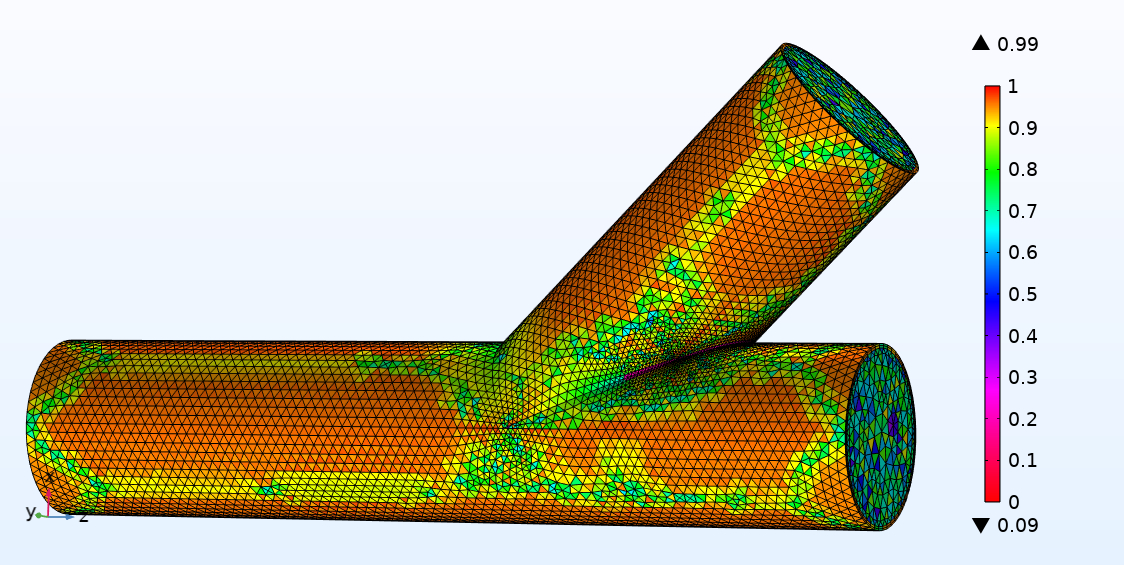
\includegraphics[width=0.88\columnwidth]{fig2_mesh.jpeg}
		\caption{Mesh.}
		\label{fig:mesh}
	\end{figure}
	
	\begin{table*}[!t]
		\centering
		\caption{Mesh analysis for the model.}
		\label{tab:mesh}
		\small
		\renewcommand{\arraystretch}{1.12}
		\begin{tabular}{lcccc}
			\hline
			\textbf{Mesh} & \textbf{Number of Elements} & \textbf{Degrees of Freedom} & \textbf{Average WBC Concentration (mol/m$^3$)} & \textbf{Variation (\%)}\\
			\hline
			Extremely Coarse & 31,287 & 156,452 & $2.051\times10^{-9}$ & ---\\
			Extra Coarse & 62,134 & 312,850 & $2.107\times10^{-9}$ & 2.65\\
			Coarser & 121,402 & 612,314 & $2.142\times10^{-9}$ & 1.90\\
			Coarse & 182,376 & 915,840 & $2.173\times10^{-9}$ & 1.80\\
			Normal & 242,890 & 1,201,563 & $2.201\times10^{-9}$ & 1.27\\
			Fine & 302,107 & 1,510,535 & $2.217\times10^{-9}$ & 0.72\\
			\hline
		\end{tabular}
	\end{table*}
	
	\section{Results and discussion}
	
	\subsection{Time dependent analysis of WBC concentration}
	
	\begin{figure}[!htbp]
		\centering
		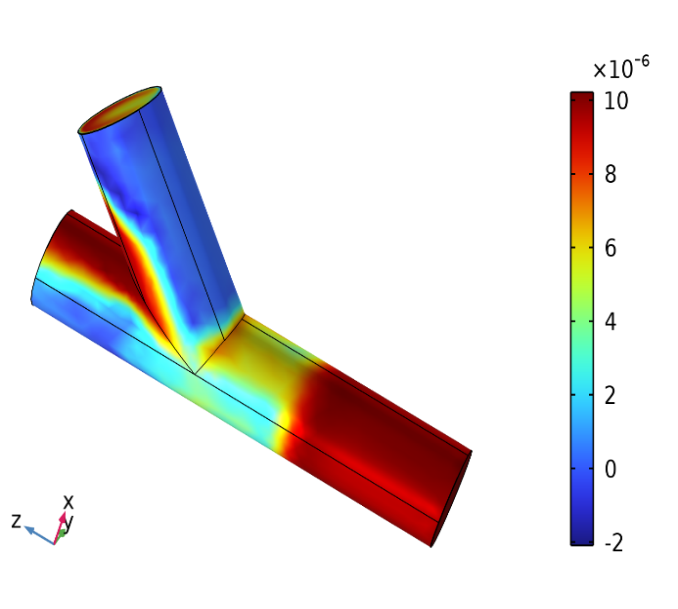
\includegraphics[width=0.48\columnwidth]{fig3_wbc_t05.png}\hfill
		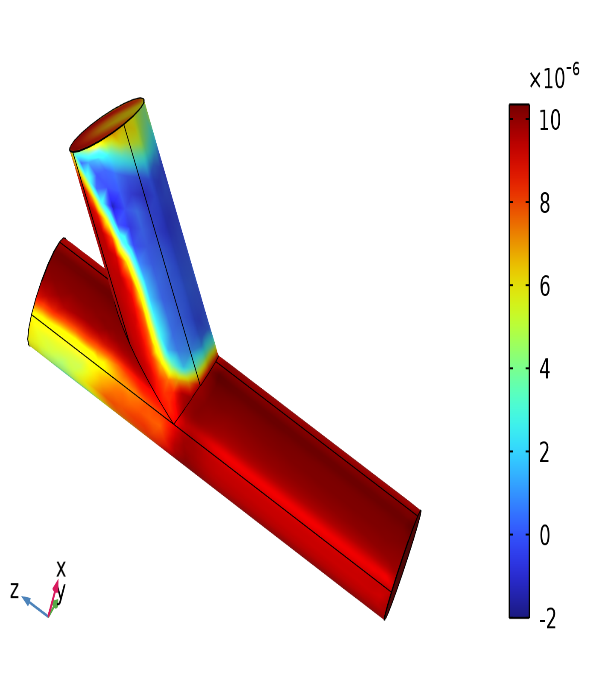
\includegraphics[width=0.48\columnwidth]{fig3_wbc_t1.png}\\[2pt]
		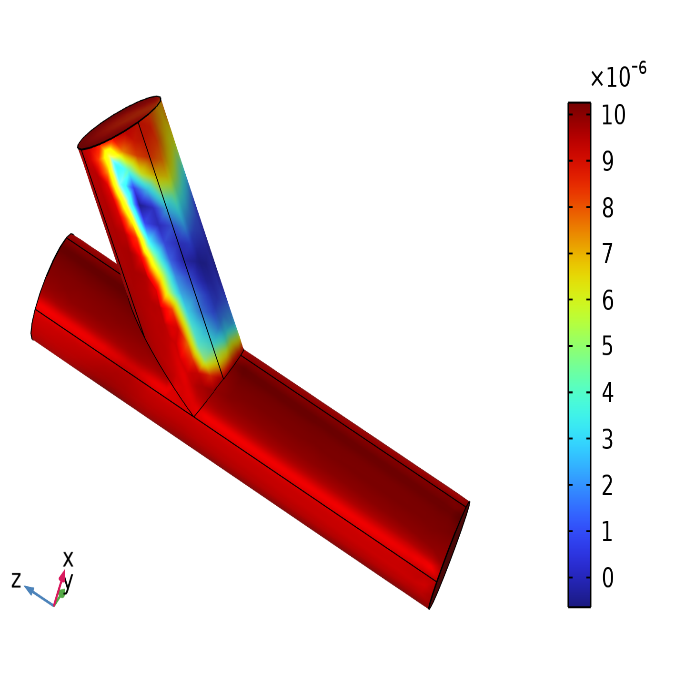
\includegraphics[width=0.48\columnwidth]{fig3_wbc_t2.png}\hfill
		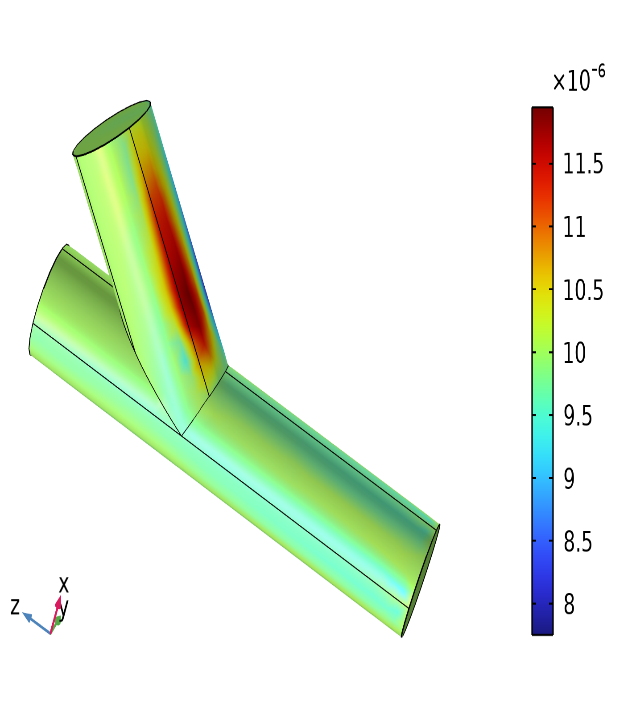
\includegraphics[width=0.48\columnwidth]{fig3_wbc_t10.png}
		\caption{WBC concentration surface plots of \feo\ nanoparticle for different time intervals $t = 0.5$\,s (top left), $t = 1$\,s (top right), $t = 2$\,s (bottom left) and $t = 10$\,s (bottom right).}
		\label{fig:wbc_time}
	\end{figure}
	
	The time-dependent analysis of WBC concentration at different time intervals (Figure~\ref{fig:wbc_time}) reveals significant trends in WBC migration, particularly around the infected portion where cytokines are released. Initial observations at $t = 0.5$\,s and $t = 1$\,s shows a progressive movement of WBCs toward the infected region, driven by the chemotactic response to the cytokine gradient. This early-stage migration shows the initial attraction phase where WBCs respond rapidly to the chemical signals, demonstrating the role of cytokine signalling in guiding immune cells. At $t = 2$\,s, there is a visible accumulation of WBCs around the infected zone, indicating a strengthened chemotactic response. However, it is at $t = 10$\,s where the concentration at the infected site reaches its peak value. This peak accumulation signifies that the WBCs continue to be attracted and held at the infected zone due to sustained cytokine release, resulting in the highest observed concentration at this point in time. On the other hand, the rest of the region shows a fairly homogeneous distribution, suggesting that WBCs far from the region of infection remain at a constant steady-state value, dependent on convection as well as basic chemotaxis.
	
	The rise in the white blood cell density observed at the site of infection after $t = 10$\,s shows how nanoparticle-assisted chemotaxis is effective in maintaining cell mobility over long periods of time. This observation is significant since it provides insights into the possible benefits of such treatments in clinical cases where specific immune responses are necessary. This consistent rise in cell density suggests how therapies can be improved where high density of cells at certain regions is needed.
	\newpage
	\subsection{Chemotactic Sensitivity Analysis of WBCs}
	
	\begin{figure}[!htbp]
		\centering
		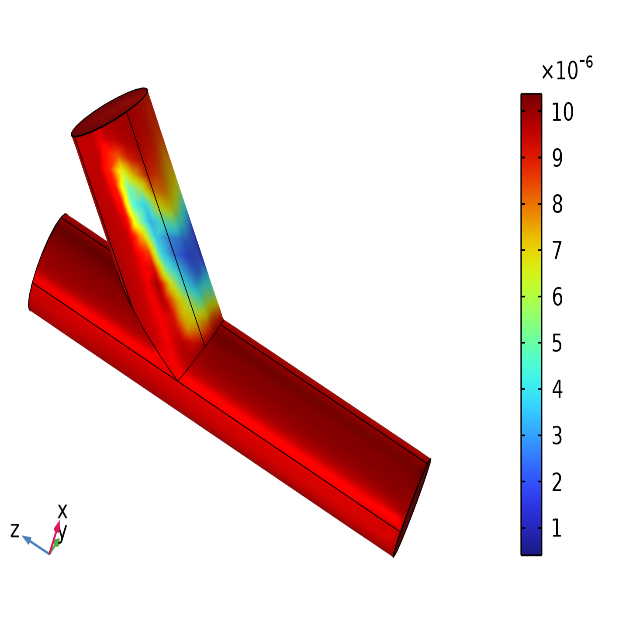
\includegraphics[width=0.48\columnwidth]{fig4_chemo_01.png}\hfill
		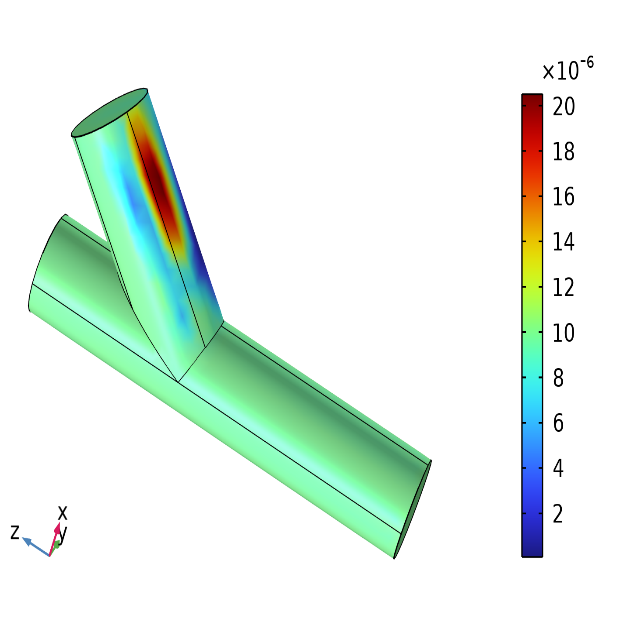
\includegraphics[width=0.48\columnwidth]{fig4_chemo_1.png}
		\caption{Effect of Chemotaxis Constant on WBC Concentration for \feo\ Nanoparticles at $t = 2$\,s for $\chi = 0.1$ and $\chi = 1$.}
		\label{fig:chemo_surface}
	\end{figure}
	
	\begin{figure}[!htbp]
		\centering
		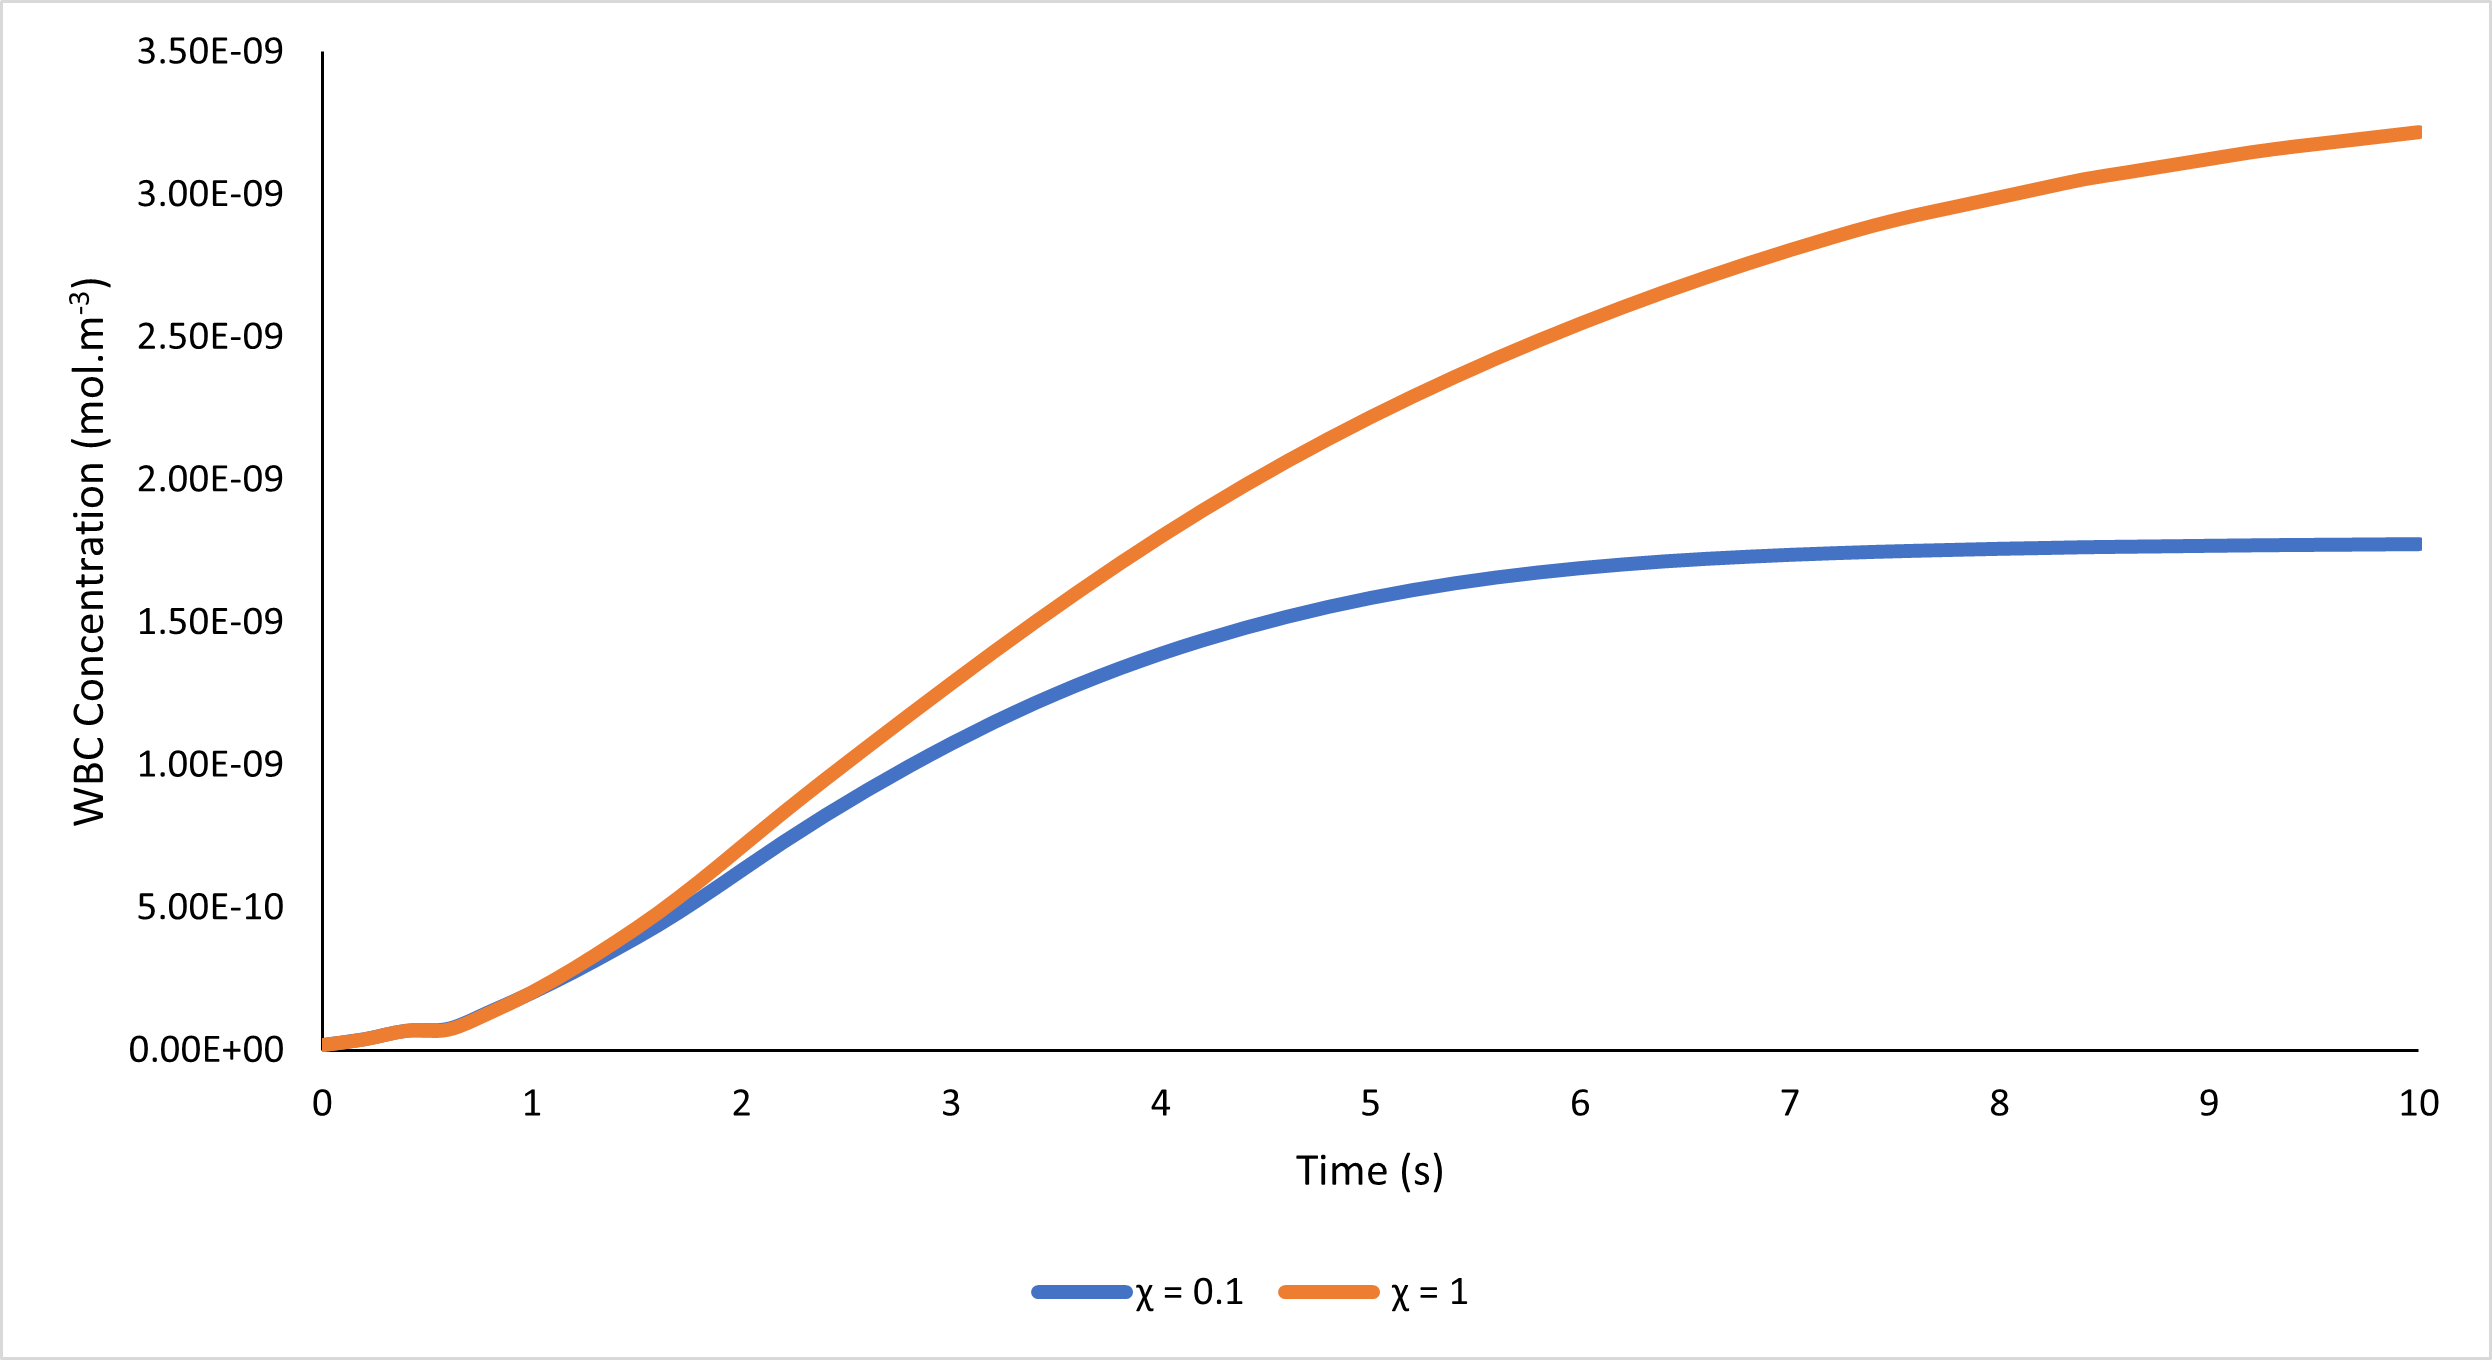
\includegraphics[width=0.88\columnwidth]{fig5_chemo_series.png}
		\caption{WBC concentration plots with varying chemotaxis constant.}
		\label{fig:chemo_series}
	\end{figure}
	
	The chemotactic sensitivity of WBCs, as shown in Figures~\ref{fig:chemo_surface} and~\ref{fig:chemo_series}, shows how the WBC concentration changes under different chemotaxis constants while considering the impact of the \feo\ particles. Figure~\ref{fig:chemo_surface} shows surface graphs for WBC distribution when $t = 2$\,s and reveals that WBCs exhibit an intermediate aggregate level near the infected area where cytokines exist. At this point, it is clear from the figures that increased chemotaxis constants result in increased gradient levels; therefore, higher chemotactic sensitivity leads to higher directed migration towards the infected areas. Figure~\ref{fig:chemo_series} displays WBC concentrations over a longer time period in which WBC behavior and migration trends have been considered based on the value of chemotaxis constant ($\chi$). The results suggest that increased $\chi$ values result in high WBC concentration levels in the infected zones. It becomes apparent that WBC concentration peaks occur at $t \approx 10$\,s, indicating that chemotactic sensitivity plays a significant role in WBC migration. Overall, it is clear from the temporal analysis that $\chi$ affects the directed migration of WBCs towards areas releasing cytokines.
	
	This suggests that it is extremely important to ensure that the chemotaxis parameter is maximized to allow immune cells to migrate and accumulate in infected areas. This shows how significant the sensitivity to chemotaxis is to ensure a locally increased concentration of white blood cells, which is crucial in ensuring efficient immune responses. Through appropriate manipulation of $\chi$, medical approaches can be optimized to improve their targeting efficiency, which may aid in developing innovative therapies for inflammation and local infections.
	
	\subsection{Modulation of WBC Concentration by Magnetic Fields Using \feo\ Nanoparticles}
	
\begin{figure}[!htbp]
	\centering
	\begin{tabular}{@{}c@{\hspace{0.02\columnwidth}}c@{}}
		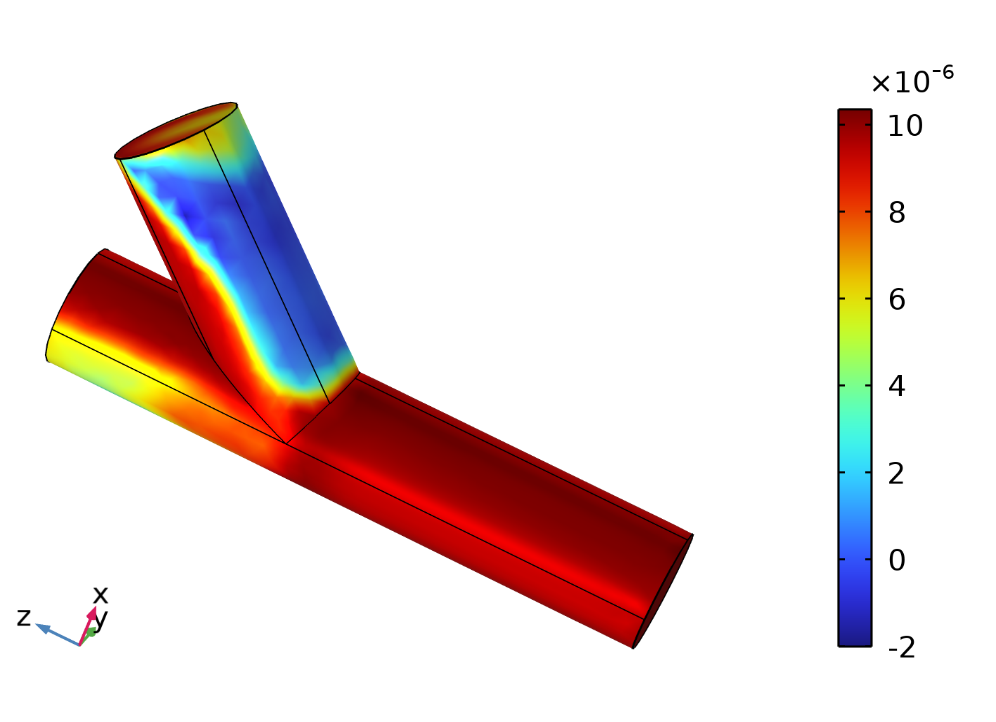
\includegraphics[width=0.5\columnwidth]{fig6_B0_full.png} &
		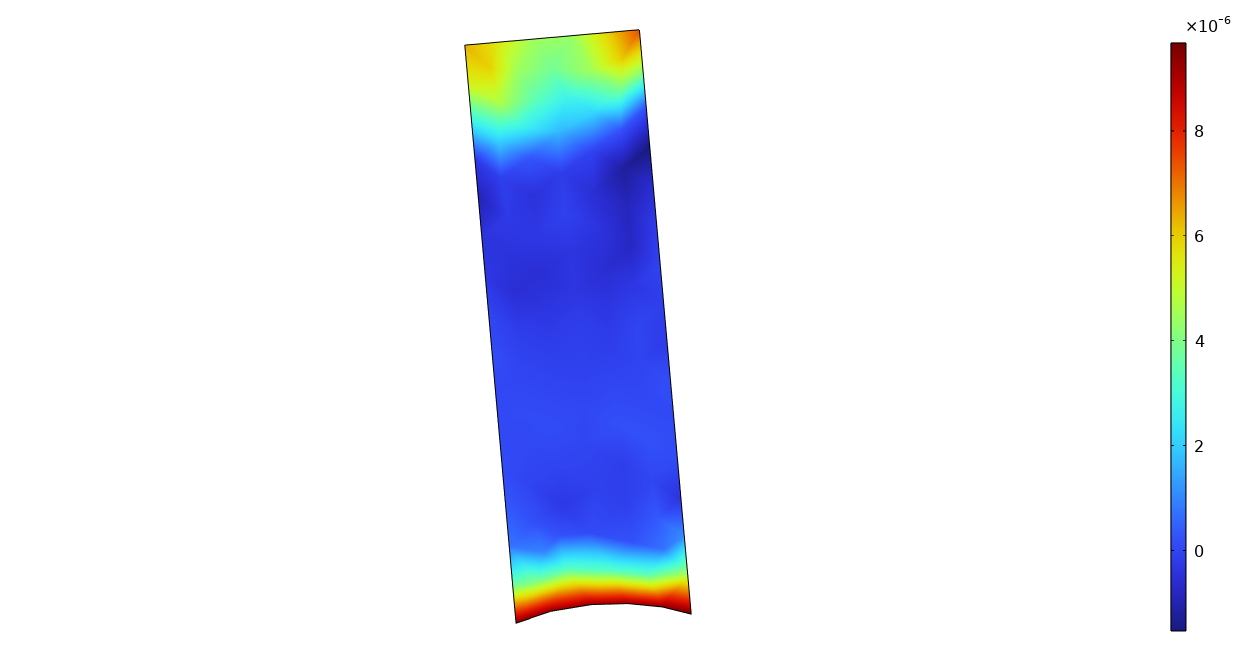
\includegraphics[width=0.5\columnwidth]{fig6_B0_infected.jpg} \\[3pt]
		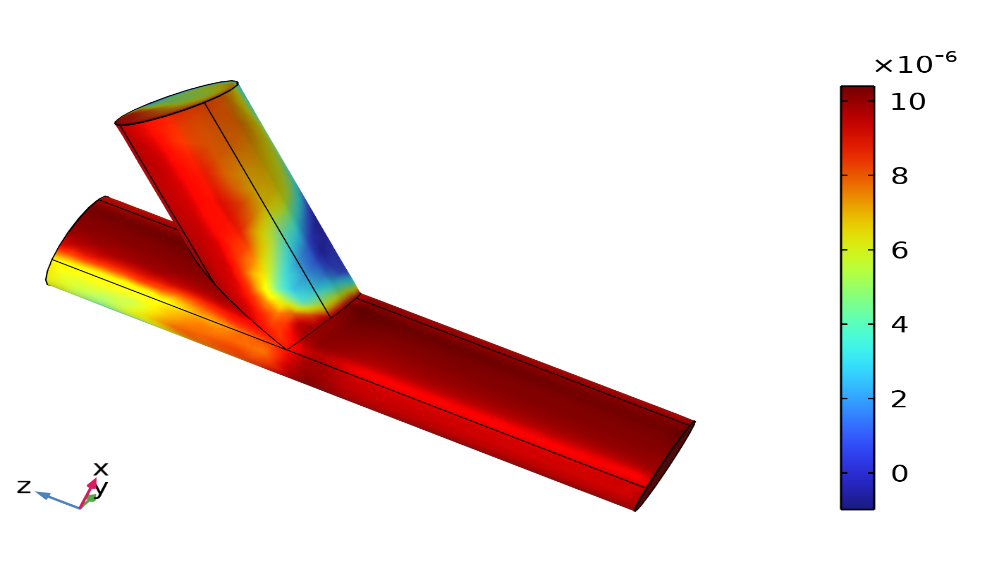
\includegraphics[width=0.5\columnwidth]{fig6_B100_full.png} &
		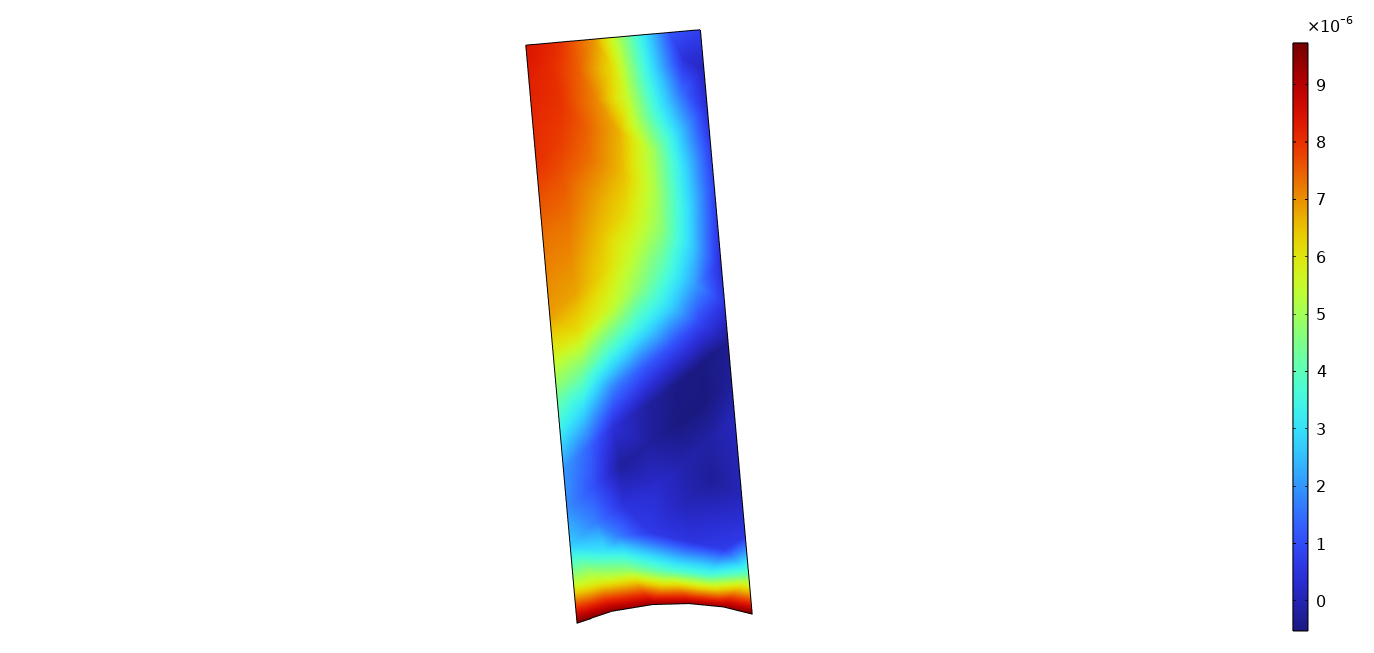
\includegraphics[width=0.5\columnwidth]{fig6_B100_infected.jpg}
	\end{tabular}
	\caption{Surface concentration plots of WBCs, showing distribution across the full model domain (left) and the infected region (right) for $B = 0$\,T (top) and $B = 100$\,T (bottom) at $t=1$\,s.}
	\label{fig:magnetic}
\end{figure}

The effect of magnetic field modulation on WBC concentration is presented in Figure~\ref{fig:magnetic}, showing distribution across the full model domain and the infected region under magnetic field. Without the presence of any external magnetic field ($B = 0$\,T), the distribution of WBCs is quite dispersed. On the other hand, in the case of a magnetic field of $100$\,T, WBCs have a high degree of aggregation around the infected area, suggesting that a magnetic navigation process plays a crucial part in WBC migration. This phenomenon of increased localization around infected areas can be explained by the effect of both the \feo\ nanoparticles and the applied magnetic field. Based on this observation, it can be said that external magnetic fields can guide WBC movements and hence, can provide precise control over such immune-related activities. Leveraging such approaches could advance treatment protocols, particularly for conditions that require precise immune cell localization, facilitating better-targeted and more efficient therapeutic outcomes.


%
\subsection{Comparative Temperature Dynamics in the Infected Region with Different Nanoparticles}

\begin{figure}[!htbp]
%	\hspace*{-1cm}%
	\begin{tabular}{@{}c@{\hspace{0.02\columnwidth}}c@{\hspace{0.02\columnwidth}}c@{}}
		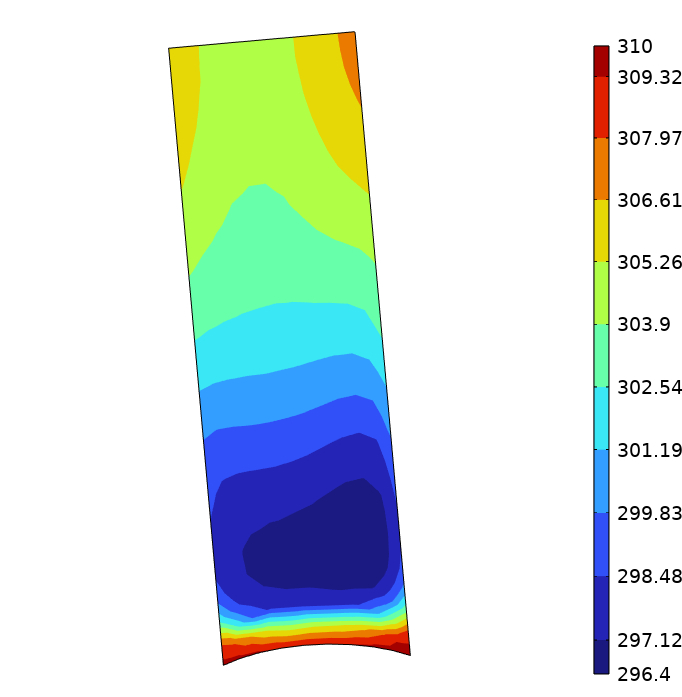
\includegraphics[width=0.30\columnwidth]{fig7a_B0_Fe3O4.jpg} &
		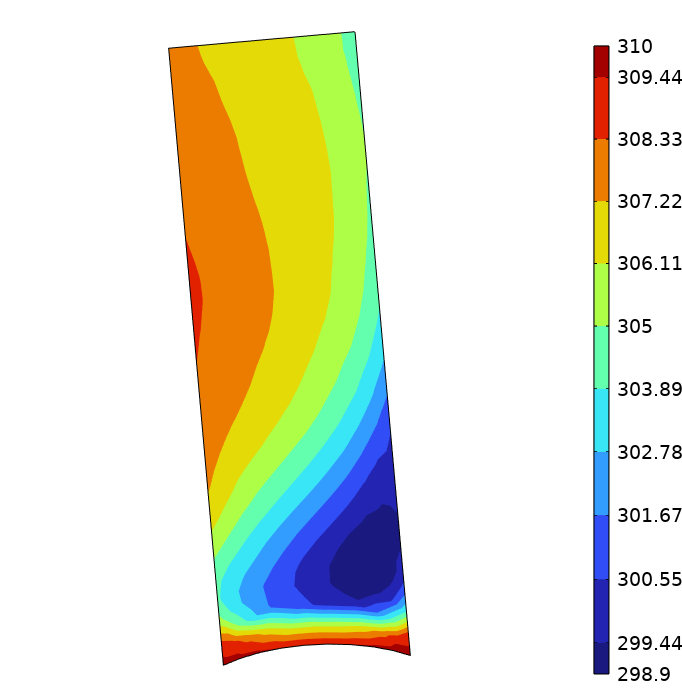
\includegraphics[width=0.30\columnwidth]{fig7b_B100_Fe3O4.jpg} &
		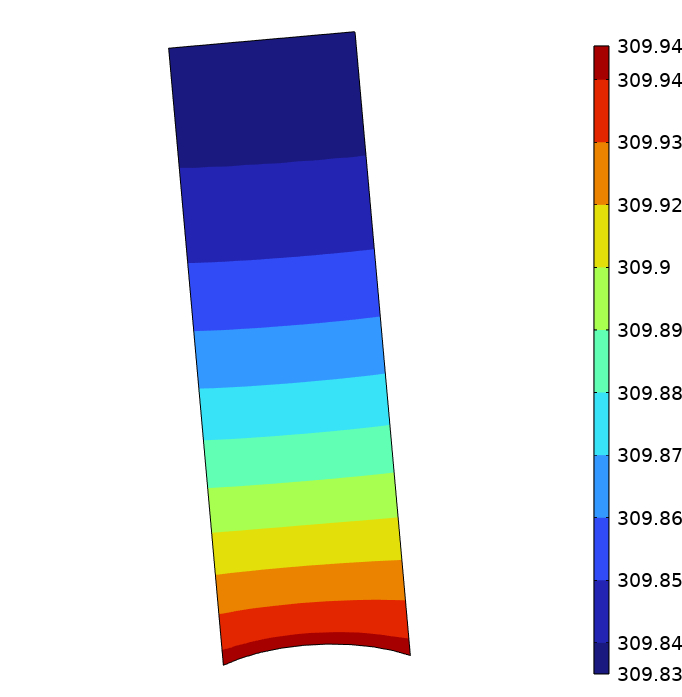
\includegraphics[width=0.30\columnwidth]{fig7c_SWCNT.jpg} \\[2pt]
		\scriptsize (a) $B = 0$\,T $(\feo)$ &
		\scriptsize (b) $B = 100$\,T $(\feo)$ &
		\scriptsize (c) $B = 0, 100$\,T $(SWCNT)$
	\end{tabular}
	
	\vspace{5pt}
	
	\hspace*{1.5cm}\parbox{\dimexpr\linewidth-1.5cm\relax}{\caption{Isothermal contours of \feo\ and SWCNT nanoparticles with varying magnetic field at the infected region for $t = 1$\,s.}
		\label{fig:isothermal}}
\end{figure}



\begin{figure}[!htbp]
	\centering
	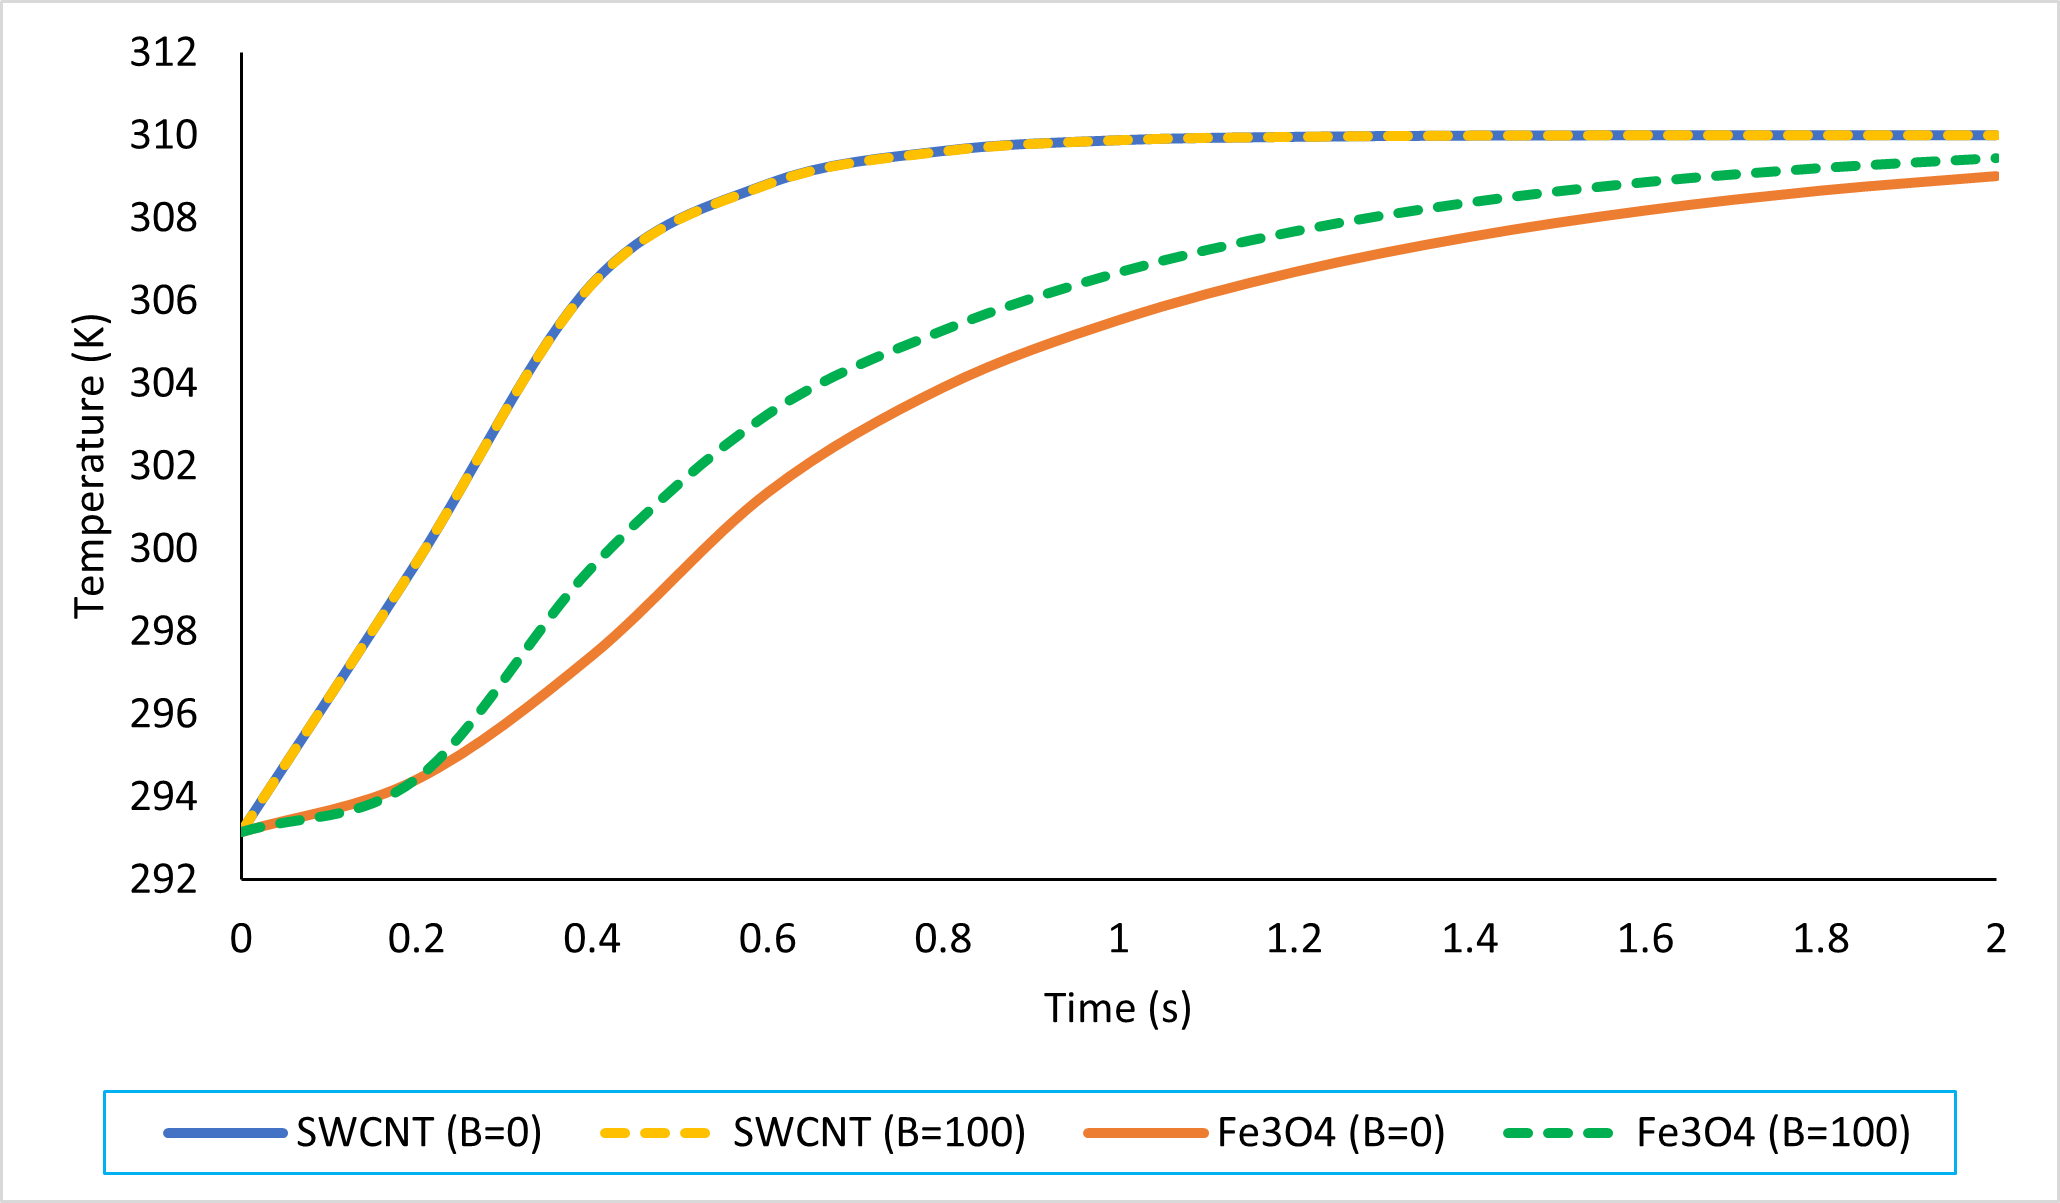
\includegraphics[width=0.88\columnwidth]{fig8_temp.png}
	\caption{Temperature distribution for \feo\ and SWCNT under varying magnetic field.}
	\label{fig:temperature}
\end{figure}
	
	Figure~\ref{fig:isothermal} illustrates the isothermal contours for temperature distribution in the infected region when using \feo\ and SWCNT nanoparticles under magnetic field conditions of $B = 0$\,T and $B = 100$\,T. For \feo\ at $B = 0$\,T, the contours display moderate thermal gradients, indicating a steady heat distribution. When a magnetic field of $B = 100$\,T is applied, the contours reveal steeper gradients, showing an increase in temperature due to \feo's magnetic properties that enhances localized heat conduction. This demonstrates \feo\ nanoparticles' capacity for leveraging magnetic fields to improve temperature variation in the targeted area.
	
	There is almost no difference in the behaviour of the isothermal contour for the SWCNT nanoparticles at different values of magnetic field strength from $B = 0$\,T to $B = 100$\,T, suggesting that magnetic fields have almost no impact here. However, since SWCNT nanoparticles are highly thermally conductive, they can help achieve uniform heating of the area. Hence, SWCNT nanoparticles are beneficial in maintaining the heat flow process; however, there is no advantage of using them when magnetic fields are involved, unlike \feo.
	
	The results demonstrate the unique thermal properties associated with the nanoparticles being discussed. As previously mentioned, single walled carbon nanotubes (SWCNTs) are ideal for uses where the need exists for an efficient and constant heat transfer process that does not involve any form of magnetic field manipulation. On the other hand, since \feo\ nanoparticles can be used in a magnetic field, they are therefore better suited in situations where the need exists for a controlled amount of temperature change. Ultimately, the choice of nanoparticle should align with the specific requirements of thermal management and magnetic field interaction to optimize therapeutic outcomes.
	
	\subsection{WBC concentration trends for different nanoparticles at the infected region under the influence of magnetic field}
	
	\begin{figure}[!htbp]
		\centering
		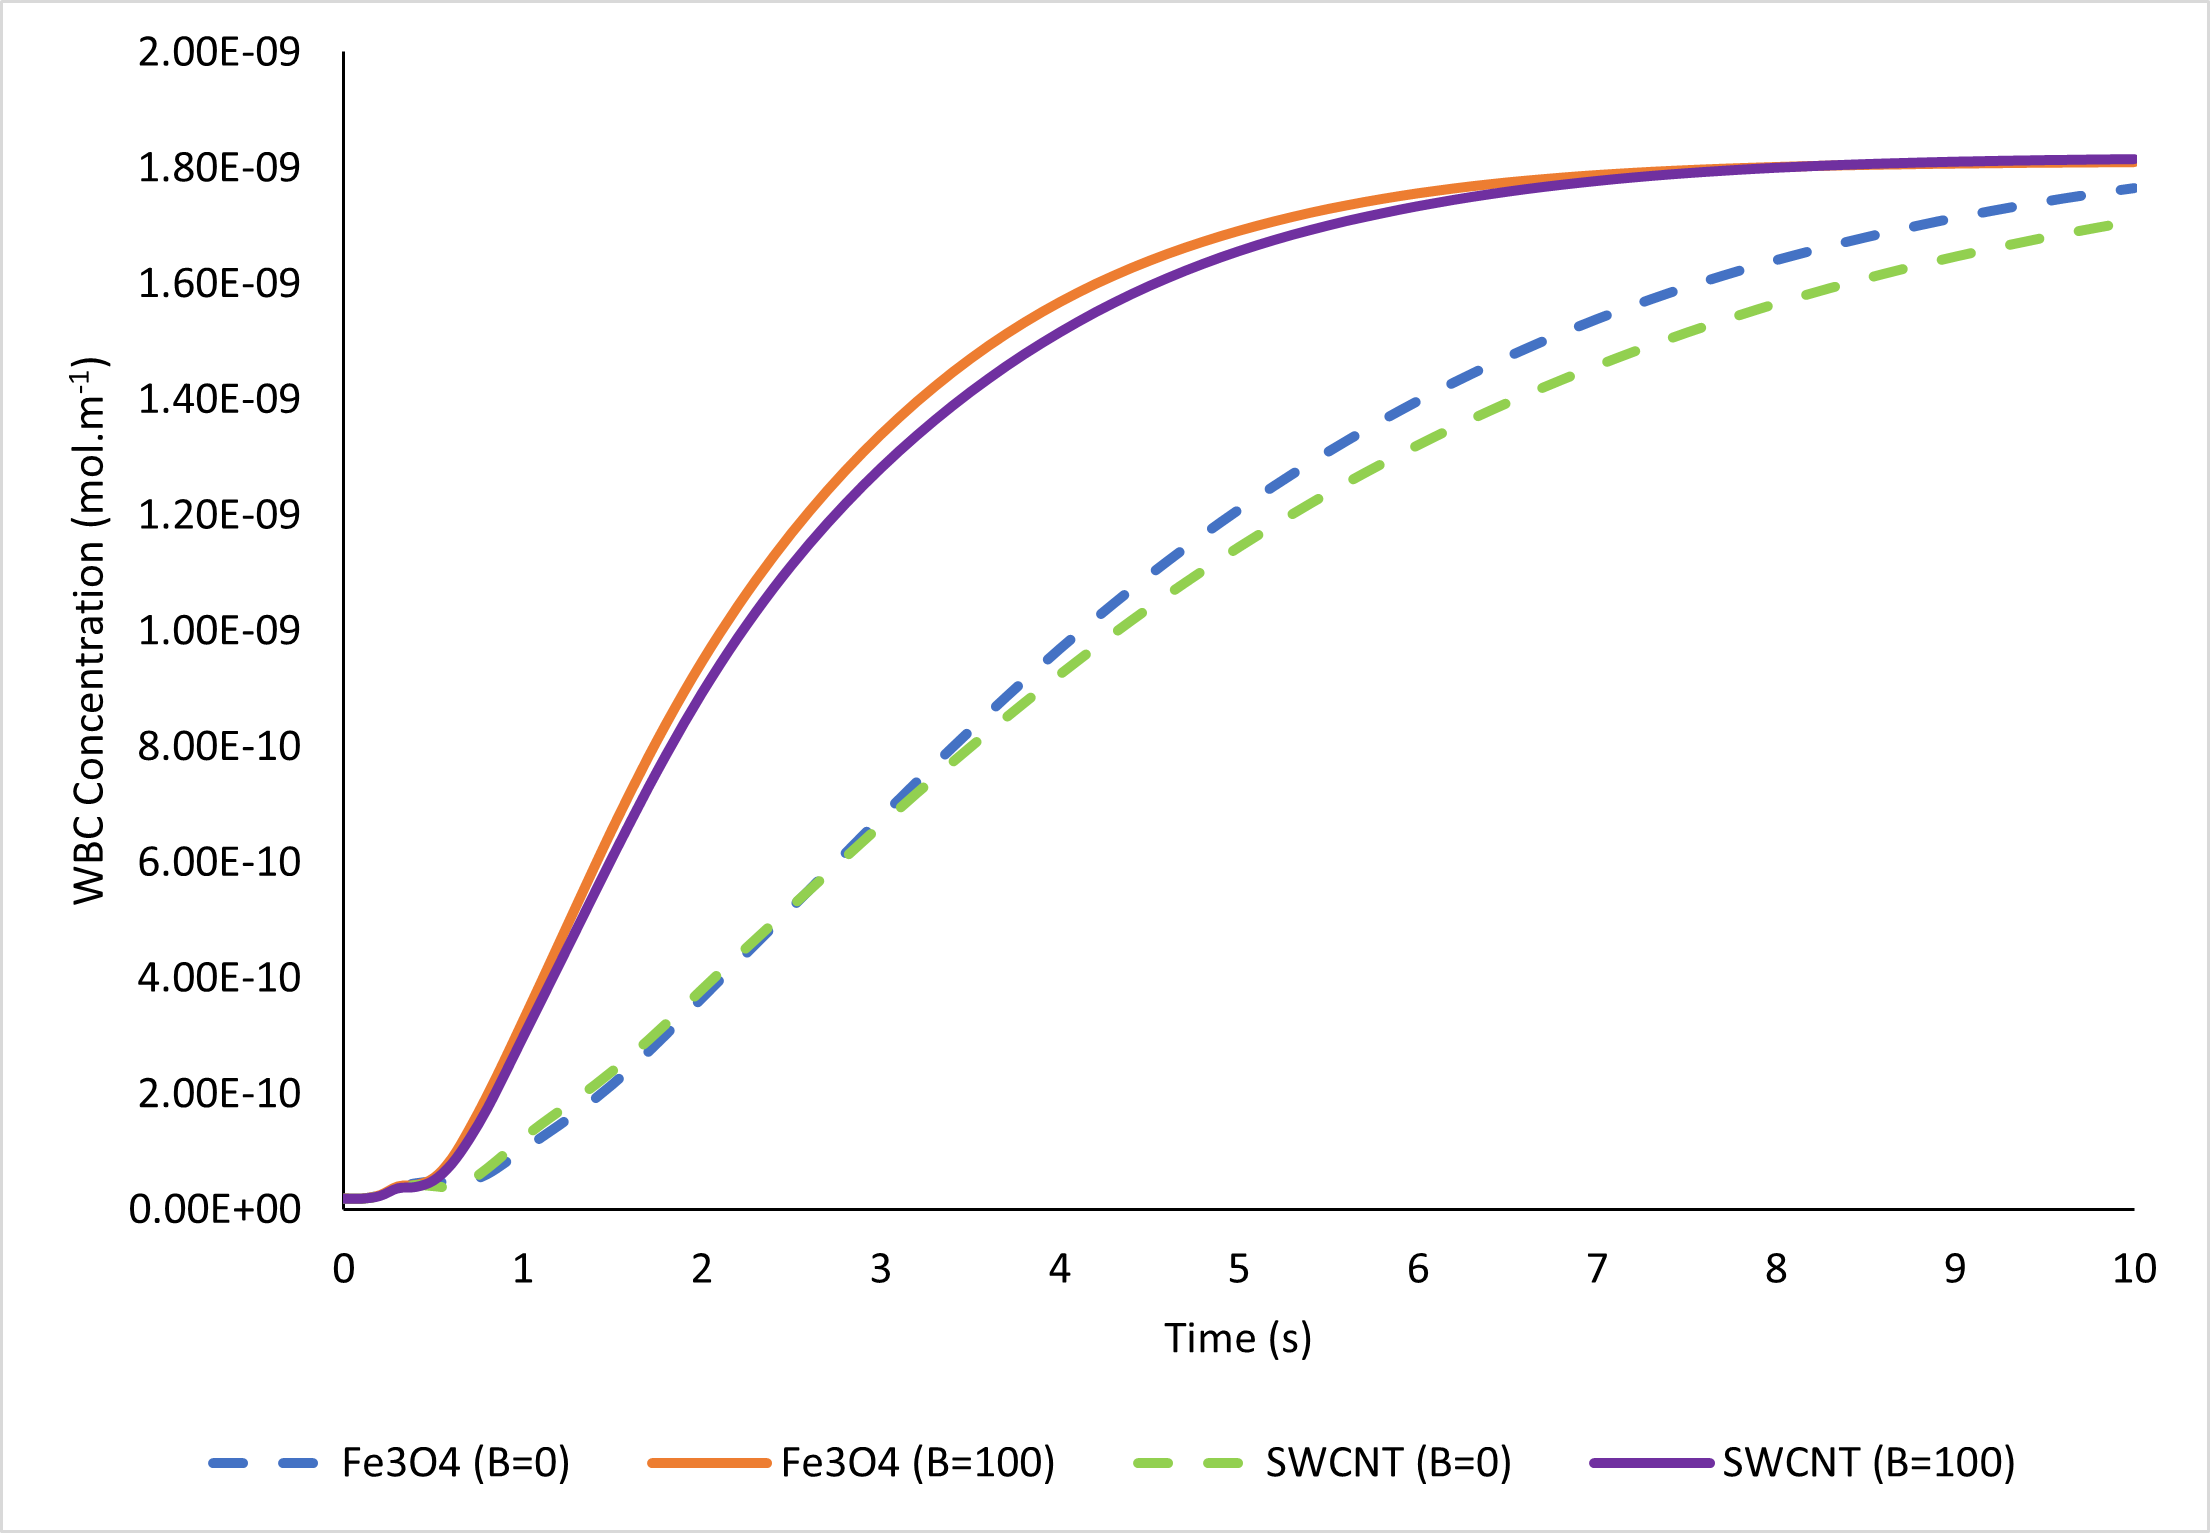
\includegraphics[width=0.88\columnwidth]{fig9_wbc_avg.png}
		\caption{Average WBC concentration distribution for \feo\ and SWCNT under varying magnetic field at the infected region.}
		\label{fig:wbc_avg}
	\end{figure}
	
	Graphical depiction of time trends for the concentration of WBC in the infected area when the nanoparticles of \feo\ and single walled carbon nanotubes (SWCNTs) are exposed to different magnetic field strengths ($B = 0$\,T and $B = 100$\,T) is shown in Figure~\ref{fig:wbc_avg}. In the case of the \feo\ nanoparticle, the trend depicts an increase in the concentration of WBC due to exposure to a magnetic field. In fact, the trend line depicting $B = 100$\,T shows faster growth of WBC concentration compared to the line for $B = 0$\,T.
	
	SWCNT nanoparticles, on the other hand, show a different pattern. The WBC concentration for SWCNT at $B = 100$\,T is higher than at $B = 0$\,T, confirming that the application of a magnetic field does affect WBC migration. However, the difference between the two curves is less pronounced than for \feo, indicating that SWCNTs' response to magnetic influence is moderate. This behavior suggests that while SWCNTs can facilitate WBC accumulation and benefit from magnetic fields to a certain extent, their enhancement is not as substantial as that of \feo.
	
	The above results demonstrate the advantages of using \feo\ nanoparticles for applications where there is a need for significant enhancement in chemotaxis due to the presence of magnetic field, hence making it an efficient material for enhancing immune cell targeting in therapy. Although SWCNTs react to magnetic fields, their efficiency would be higher when applied in applications that require consistency rather than enhancement.
	
	\section{Conclusion}
	
	A full mathematical model was created to analyze the process of blood flow, leukocyte movement, nanoparticle transport, and cytokines interaction under influence of magnetic field, using COMSOL Multiphysics program. The present research is characterized by unique incorporation of \feo\ and SWCNT nanoparticles for studying the effect of each of them on chemotaxis and temperature distribution of leukocytes.
	
	These findings reveal that the exposure of \feo\ nanoparticles to magnetic fields significantly elevates WBCs levels at the area of infection. Thus, the implications of these discoveries are that such nanoparticles could be applied in biological processes involving the use of magnets to target immune cells. On the other hand, SWCNT nanoparticles have excellent heat conductance characteristics, resulting in a constant temperature pattern whether there is an application of a magnetic field or not. Hence, they are better suited to applications where constant temperatures are involved. The findings of this study are in line with biological phenomena.
	
	This is the progression of our comprehension of the behaviour of white blood cells and nanoparticles in blood flow. However, there are aspects in which this model is deficient and must be recognized. This study focuses on the main interactions of the white blood cells, nanoparticles, and cytokines without considering the possible effects of other immune cells as well as their biochemistry involving other cytokines. Complexities such as variable blood properties, the role of cardiac pulsatility, and real-world geometrical variations were simplified or omitted to maintain computational tractability. Additionally, while this model incorporated the magnetic responsiveness of \feo, more comprehensive studies that include varying magnetic field orientations and intensities would provide deeper insights.
	
	In general, the model that was designed helps in gaining more insight regarding the ways magnetic nanoparticles could be used to influence immune responses and manage heat distribution. Based on the findings of this investigation, it is crucial to choose a proper type of nanoparticles to achieve desired results in terms of developing therapy. In spite of certain drawbacks, the investigation provides relevant information about nanoparticle use for designing future studies on more complex models.
	
	\section*{Declarations}  
	
	\textbf{Conflict of interest:} The authors proclaim no potential conflict of interest with respect to the research, authorship and publication of this article.
	
	\begin{thebibliography}{99}
		\footnotesize
		\setlength{\itemsep}{0pt plus 0.2pt}
		\setlength{\parsep}{0pt}
		\setlength{\parskip}{0pt}
		
		\bibitem{Ku1997}
		D.N. Ku, Blood flow in arteries, Annual Review of Fluid Mechanics \textbf{29}, 399--434 (1997) DOI: \url{https://doi.org/10.1146/annurev.fluid.29.1.399}
		
		\bibitem{Zhao2000}
		S.Z. Zhao, X.Y. Xu, A.D. Hughes, S.A. Thom, A.V. Stanton, B. Ariff, Q. Long, Blood flow and vessel mechanics in a physiologically realistic model of a human carotid arterial bifurcation, Journal of Biomechanics \textbf{33}, 975--984 (2000) DOI: \url{https://doi.org/10.1016/S0021-9290(00)00043-9}
		
		\bibitem{Steinman2004}
		D.A. Steinman, Image-based computational fluid dynamics: a new paradigm for monitoring hemodynamics and atherosclerosis, Current Drug Targets-Cardiovascular \& Hematological Disorders \textbf{4}, 183--197 (2004) DOI: \url{https://doi.org/10.2174/1568006043336302}
		
		\bibitem{Singh2010}
		R. Singh, G.C. Sharma, M. Jain, Mathematical modeling of blood flow in a stenosed artery under MHD effect through porous medium, International Journal of Engineering \textbf{23}, 243--252 (2010)
		
		\bibitem{Rezazadeh2022}
		M. Rezazadeh, R. Ostadi, Numerical simulation of the wall shear stress distribution in a carotid artery bifurcation, Journal of Mechanical Science and Technology \textbf{36}, 5035--5046 (2022) DOI: \url{https://doi.org/10.1007/s12206-022-0917-9}
		
		\bibitem{Katanov2015}
		D. Katanov, G. Gompper, D.A. Fedosov, Microvascular blood flow resistance: role of red blood cell migration and dispersion, Microvascular Research \textbf{99}, 57--66 (2015) DOI: \url{https://doi.org/10.1016/j.mvr.2015.02.006}
		
		\bibitem{Milnor1989}
		W.R. Milnor, Hemodynamic, 2nd edn. (Baltimore, MD: William and Wilkins, 1989).
		
		\bibitem{Iliceto1991}
		S. Iliceto, V. Marangelli, C. Memmola, P. Rizzon, Transesophageal Doppler echocardiography evaluation of coronary blood flow velocity in baseline conditions and during dipyridamole-induced coronary vasodilation, Circulation \textbf{83}, 61--69 (1991) DOI: \url{https://doi.org/10.1161/01.cir.83.1.61}
		
		\bibitem{Shen2018}
		L. Shen, B. Li, Y. Qiao, \feo\ nanoparticles in targeted drug/gene delivery systems, Materials \textbf{11}, 324 (2018) DOI: \url{https://doi.org/10.3390/ma11020324}
		
		\bibitem{Fullstone2015}
		G. Fullstone, J. Wood, M. Holcombe, G. Battaglia, Modelling the transport of nanoparticles under blood flow using an agent-based approach, Scientific Reports \textbf{5}, 10649 (2015) DOI: \url{https://doi.org/10.1038/srep10649}
		
		\bibitem{Gentile2008}
		F. Gentile, M. Ferrari, P. Decuzzi, The transport of nanoparticles in blood vessels: the effect of vessel permeability and blood rheology, Annals of Biomedical Engineering \textbf{36}, 254--261 (2008) DOI: \url{https://doi.org/10.1007/s10439-007-9423-6}
		
		\bibitem{Ghasemi2015}
		S.E. Ghasemi, M. Hatami, A.K. Sarokolaie, D.D. Ganji, Study on blood flow containing nanoparticles through porous arteries in presence of magnetic field using analytical methods, Physica E: Low-dimensional Systems and Nanostructures \textbf{70}, 146--156 (2015) DOI: \url{https://doi.org/10.1016/j.physe.2015.03.002}
		
		\bibitem{Boujelbene2023}
		M. Boujelbene, S. Rehman, S. Alqahtani, S. Alshehery, Second law assessment of injected nanoparticles to blood flow with thermal radiation and magnetic field in conduit artery, Journal of the Taiwan Institute of Chemical Engineers \textbf{150}, 105074 (2023) DOI: \url{https://doi.org/10.1016/j.jtice.2023.105074}
		
		\bibitem{Siogkas2011}
		P. Siogkas, A. Sakellarios, T.P. Exarchos, L. Athanasiou, E. Karvounis, K. Stefanou, et al., Multiscale-patient-specific artery and atherogenesis models, IEEE Transactions on Biomedical Engineering \textbf{58}, 3464--3468 (2011) DOI: \url{https://doi.org/10.1109/tbme.2011.2164919}
		
		\bibitem{Gerhardt2015}
		T. Gerhardt, K. Ley, Monocyte trafficking across the vessel wall, Cardiovascular Research \textbf{107}, 321--330 (2015) DOI: \url{https://doi.org/10.1093/cvr/cvv147}
		
		\bibitem{Cavaillon1994}
		J.M. Cavaillon, Cytokines and macrophages, Biomedicine \& Pharmacotherapy \textbf{48}, 445--453 (1994) DOI: \url{https://doi.org/10.1016/0753-3322(94)90005-1}
		
		\bibitem{Zlotnik2000}
		A. Zlotnik, O. Yoshie, Chemokines: a new classification system and their role in immunity, Immunity \textbf{12}, 121--127 (2000) DOI: \url{https://doi.org/10.1016/s1074-7613(00)80165-x}
		
		\bibitem{Dubey2021}
		A. Dubey, B. Vasu, O.A. Bég, R.S.R. Gorla, Finite element computation of magneto-hemodynamic flow and heat transfer in a bifurcated artery with saccular aneurysm using the Carreau-Yasuda biorheological model, Microvascular Research \textbf{138}, 104221 (2021) DOI: \url{https://doi.org/10.1016/j.mvr.2021.104221}
		
		\bibitem{KhanKhan2009}
		F.H. Khan, F. Khan, The elements of immunology, Pearson Education India (2009).
		
		\bibitem{Hewlin2023}
		R.L. Hewlin Jr, M. Smith, J.P. Kizito, Computational assessment of unsteady flow effects on magnetic nanoparticle targeting efficiency in a magnetic stented carotid bifurcation artery, Cardiovascular Engineering and Technology \textbf{14}, 694--712 (2023) DOI: \url{https://doi.org/10.1007/s13239-023-00681-3}
		
		\bibitem{Anderson2013}
		M.D. Anderson, Y.F. Xiao, J.M. Fraser, First-passage theory of exciton population loss in single-walled carbon nanotubes reveals micron-scale intrinsic diffusion lengths, Physical Review B \textbf{88}, 045420 (2013) DOI: \url{https://doi.org/10.1103/physrevb.88.045420}
		
		\bibitem{Lee2010}
		H. Lee, H. Fonge, B. Hoang, R.M. Reilly, C. Allen, The effects of particle size and molecular targeting on the intra-tumoral and subcellular distribution of polymeric nanoparticles, Molecular Pharmaceutics \textbf{7}, 1195--1208 (2010) DOI: \url{https://doi.org/10.1021/mp100038h}
		
		\bibitem{Sha2017}
		L. Sha, Y. Ju, H. Zhang, The influence of the magnetic field on the convective heat transfer characteristics of \feo/water nanofluids, Applied Thermal Engineering \textbf{126}, 108--116 (2017) DOI: \url{https://doi.org/10.1016/j.applthermaleng.2017.07.150}
		
		\bibitem{Wei2018}
		X. Wei, L. Jing, C. Liu, Y. Hou, M. Jiao, M. Gao, Molecular mechanisms for delicately tuning the morphology and properties of \feo\ nanoparticle clusters, CrystEngComm \textbf{20}, 2421--2429 (2018) DOI: \url{https://doi.org/10.1039/c8ce00056e}
		
		\bibitem{Muhammad2018}
		S. Muhammad, G. Ali, Z. Shah, S. Islam, S.A. Hussain, The rotating flow of magneto hydrodynamic carbon nanotubes over a stretching sheet with the impact of non-linear thermal radiation and heat generation/absorption, Applied Sciences \textbf{8}, 482 (2018) DOI: \url{https://doi.org/10.3390/app8040482}
		
		\bibitem{Budu2008}
		P. Budu-Grajdeanu, R.C. Schugart, A. Friedman, C. Valentine, A.K. Agarwal, B.H. Rovin, A mathematical model of venous neointimal hyperplasia formation, Theoretical Biology and Medical Modelling \textbf{5}, 1--9 (2008) DOI: \url{https://doi.org/10.1186/1742-4682-5-2}
		
		\bibitem{Cilla2014}
		M. Cilla, E. Pena, M.A. Martinez, Mathematical modelling of atheroma plaque formation and development in coronary arteries, Journal of The Royal Society Interface \textbf{11}, 20130866 (2014) DOI: \url{https://doi.org/10.1098/rsif.2013.0866}
		
		\bibitem{Menon2024}
		K. Menon, Z. Hu, A.L. Marsden, Cardiovascular fluid dynamics: a journey through our circulation, Flow \textbf{4}, E7 (2024) DOI: \url{https://doi.org/10.1017/flo.2024.5}
		
		\bibitem{Ali2021}
		F. Ali, S. Majeed, A. Imtiaz, Magnetohydrodynamic blood flow in a cylindrical tube with magnetic particles: a time fractional model, Mathematical Problems in Engineering \textbf{2021}, 6624912 (2021) DOI: \url{https://doi.org/10.1155/2021/6624912}
		
		\bibitem{Majeed2022}
		S. Majeed, F. Ali, A. Imtiaz, I. Khan, M. Andualem, Fractional model of MHD blood flow in a cylindrical tube containing magnetic particles, Scientific Reports \textbf{12}, 418 (2022) DOI: \url{https://doi.org/10.1038/s41598-021-04088-9}
		
		\bibitem{Vaidya2021}
		H. Vaidya, C. Rajashekhar, K.V. Prasad, S.U. Khan, F. Mebarek-Oudina, A. Patil, P. Nagathan, Channel flow of MHD bingham fluid due to peristalsis with multiple chemical reactions: an application to blood flow through narrow arteries, SN Applied Sciences \textbf{3}, 1--12 (2021) DOI: \url{https://doi.org/10.1007/s42452-021-04143-0}
		
		\bibitem{Ougrinovskaia2010}
		A. Ougrinovskaia, R.S. Thompson, M.R. Myerscough, An ODE model of early stages of atherosclerosis: mechanisms of the inflammatory response, Bulletin of Mathematical Biology \textbf{72}, 1534--1561 (2010) DOI: \url{https://doi.org/10.1007/s11538-010-9509-4}
		
		\bibitem{AhmedMishra2026}
		S. Ahmed, S.R. Mishra, Magneto-responsive hemodynamic behaviour of nanofuids in biomedical transport: a multiphysics design approach and artificial neural network predictions, International Journal of Mechanics and Materials in Design \textbf{22}, 106 (2026) DOI: \url{https://doi.org/10.1007/s10999-026-09931-3}
		
		\bibitem{Maxwell1873}
		J.C. Maxwell, A Treatise on Electricity and Magnetism, Clarendon Press, Oxford (1873).
		
		\bibitem{Brinkman1952}
		H.C. Brinkman, The viscosity of concentrated suspensions and solutions, Journal of Chemical Physics \textbf{20}, 571--581 (1952) DOI: \url{https://doi.org/10.1063/1.1700493}
		
	\end{thebibliography}
	
\end{document}
